%----------------------------------------------------------------------------------------
%	PACKAGES AND OTHER DOCUMENT CONFIGURATIONS
%----------------------------------------------------------------------------------------

\documentclass[
    11pt,
%oneside, % Two side (alternating margins) for binding by default, uncomment to switch to one side
    english, % ngerman for German
    singlespacing, % Single line spacing, alternatives: onehalfspacing or doublespacing
%draft, % Uncomment to enable draft mode (no pictures, no links, overfull hboxes indicated)
%nolistspacing, % If the document is onehalfspacing or doublespacing, uncomment this to set spacing in lists to single
%liststotoc, % Uncomment to add the list of figures/tables/etc to the table of contents
%toctotoc, % Uncomment to add the main table of contents to the table of contents
%parskip, % Uncomment to add space between paragraphs
%nohyperref, % Uncomment to not load the hyperref package
    headsepline, % Uncomment to get a line under the header
%chapterinoneline, % Uncomment to place the chapter title next to the number on one line
%consistentlayout, % Uncomment to change the layout of the declaration, abstract and acknowledgements pages to match the default layout
    oneside, % uncomment for clear page spacing between sections
]{MastersDoctoralThesis} % The class file specifying the document structure

\usepackage[utf8]{inputenc} % Required for inputting international characters
\usepackage[T1]{fontenc} % Output font encoding for international characters
\usepackage{float}% If comment this, figure moves to Page 2
\usepackage{spverbatim}

\usepackage{mathpazo} % Use the Palatino font by default

\usepackage[backend=bibtex,style=authoryear,natbib=true]{biblatex} % Use the bibtex backend with the authoryear citation style (which resembles APA)

\addbibresource{main.bib} % The filename of the bibliography

\usepackage[autostyle=true]{csquotes} % Required to generate language-dependent quotes in the bibliography


%----------------------------------------------------------------------------------------
%	MARGIN SETTINGS
%----------------------------------------------------------------------------------------

\geometry{
    paper=a4paper, % Change to letterpaper for US letter
    inner=2.5cm, % Inner margin
    outer=3.8cm, % Outer margin
    bindingoffset=.5cm, % Binding offset
    top=1.5cm, % Top margin
    bottom=1.5cm, % Bottom margin
%showframe, % Uncomment to show how the type block is set on the page
}

%----------------------------------------------------------------------------------------
%	THESIS INFORMATION
%----------------------------------------------------------------------------------------

\thesistitle{The Mango Messenger} % Your thesis title, this is used in the title and abstract, print it elsewhere with \ttitle
\supervisor{Dr. Szymon Murawski} % Your supervisor's name, this is used in the title page, print it elsewhere with \supname
\examiner{} % Your examiner's name, this is not currently used anywhere in the template, print it elsewhere with \examname
\degree{Bachelor of Computer Science} % Your degree name, this is used in the title page and abstract, print it elsewhere with \degreename
\author{Petro Kolosov, Serhii Holishevskyi, Illia Zubachov, Arslanbek Temirbekov} % Your name, this is used in the title page and abstract, print it elsewhere with \authorname
\addresses{} % Your address, this is not currently used anywhere in the template, print it elsewhere with \addressname

\subject{Biological Sciences} % Your subject area, this is not currently used anywhere in the template, print it elsewhere with \subjectname
\keywords{} % Keywords for your thesis, this is not currently used anywhere in the template, print it elsewhere with \keywordnames
\university{Wyzsza Szkola Bankowa w Poznaniu} % Your university's name and URL, this is used in the title page and abstract, print it elsewhere with \univname
\department{Department of Computer Science} % Your department's name and URL, this is used in the title page and abstract, print it elsewhere with \deptname
\group{Wyzsza Szkola Bankowa w Poznaniu} % Your research group's name and URL, this is used in the title page, print it elsewhere with \groupname
\faculty{Computer Science} % Your faculty's name and URL, this is used in the title page and abstract, print it elsewhere with \facname

\AtBeginDocument{
    \hypersetup{pdftitle=\ttitle} % Set the PDF's title to your title
    \hypersetup{pdfauthor=\authorname} % Set the PDF's author to your name
    \hypersetup{pdfkeywords=\keywordnames} % Set the PDF's keywords to your keywords
}

\begin{document}

    \frontmatter % Use roman page numbering style (i, ii, iii, iv...) for the pre-content pages

    \pagestyle{plain} % Default to the plain heading style until the thesis style is called for the body content

%----------------------------------------------------------------------------------------
%	TITLE PAGE
%----------------------------------------------------------------------------------------

    \begin{titlepage}
        \begin{center}
            
\includegraphics[width=0.5\textwidth]{Pictures/wsb_logo} \\ % University/department logo - uncomment to place it
            \vspace*{.06\textheight}
            {\scshape\LARGE \univname\par}\vspace{1.5cm} % University name
            \textsc{\Large Bachelor Thesis}\\[0.5cm] % Thesis type

            \HRule \\[0.4cm] % Horizontal line
            {\huge \bfseries \ttitle\par}\vspace{0.4cm}
            \HRule \\[1.5cm] % Horizontal line

            \begin{minipage}[t]{0.4\textwidth}
                \begin{flushleft}
                    \large
                    \emph{Authors:}\\
                    \authorname % Author name - remove the \href bracket to remove the link
                \end{flushleft}
            \end{minipage}
            \begin{minipage}[t]{0.4\textwidth}
                \begin{flushright}
                    \large
                    \emph{Supervisor:} \\
                    \supname % Supervisor name - remove the \href bracket to remove the link
                \end{flushright}
            \end{minipage}\\[3cm]

            \vfill

            \large \textit{A thesis submitted in fulfillment of the requirements\\ for the degree of \degreename}\\[0.3cm] % University requirement text
            \textit{in the}\\[0.4cm]
            \groupname\\\deptname\\[2cm] % Research group name and department name

            \vfill

            {\large \today}\\[4cm] % Date

            \vfill
        \end{center}
    \end{titlepage}

%----------------------------------------------------------------------------------------
%	DECLARATION PAGE
%----------------------------------------------------------------------------------------

    \begin{declaration}
        \addchaptertocentry{\authorshipname} % Add the declaration to the table of contents
        \noindent We, \authorname, declare that this thesis titled, \enquote{\ttitle} and the work presented in it are our own.
        We confirm that:

        \begin{itemize}
            \item This work was done wholly or mainly while in candidature for a research degree at WSB in Poznan University.
            \item Where any part of this thesis has previously been submitted for a degree or any other qualification
            at this University or any other institution, this has been clearly stated.
            \item Where We have consulted the published work of others, this is always clearly attributed.
            \item Where We have quoted from the work of others, the source is always given.
            With the exception of such quotations, this thesis is entirely our own work.
            \item We have acknowledged all main sources of help.
            \item Where the thesis is based on work done by ourselves jointly with others,
            We have made clear exactly what was done by others and what I have contributed myself.\\
        \end{itemize}

        \noindent Signed: \\
        \rule[0.5em]{25em}{0.5pt} % This prints a line for the signature

        \noindent Date: \\
        \rule[0.5em]{25em}{0.5pt} % This prints a line to write the date
    \end{declaration}

%----------------------------------------------------------------------------------------
%	PARTNER DETAILS PAGE
%----------------------------------------------------------------------------------------
    \begin{partnerdetailspage}
        \textbf{Mentor's details} \\

        \begin{tabular}{|p{5cm}|p{5cm}|}
            \hline
            First name and surname & Szymon Murawski \\
            \hline
            Degree                 &                 \\
            \hline
            Date and signature     &                 \\
            \hline
            \multicolumn{2}{c}{\vspace{0.5cm}} \\
        \end{tabular}

        \textbf{Team members' details} \\

        \begin{tabular}{|p{5cm}|p{5cm}|}
            \hline
            First name and surname & Petro Kolosov        \\
            \hline
            Course of study        &                      \\
            \hline
            Type of study program  &                      \\
            \hline
            Date and signature     &                      \\
            \hline

            \multicolumn{2}{c}{\vspace{0.5cm}} \\

            \hline
            First name and surname & Serhii Holishevskyi  \\
            \hline
            Course of study        &                      \\
            \hline
            Type of study program  &                      \\
            \hline
            Date and signature     &                      \\
            \hline

            \multicolumn{2}{c}{\vspace{0.5cm}} \\

            \hline
            First name and surname & Illia Zubachov       \\
            \hline
            Course of study        &                      \\
            \hline
            Type of study program  &                      \\
            \hline
            Date and signature     &                      \\
            \hline

            \multicolumn{2}{c}{\vspace{0.5cm}} \\

            \hline
            First name and surname & Arslanbek Temirbekov \\
            \hline
            Course of study        &                      \\
            \hline
            Type of study program  &                      \\
            \hline
            Date and signature     &                      \\
            \hline
        \end{tabular}
    \end{partnerdetailspage}

    \clearpage
%----------------------------------------------------------------------------------------
%	QUOTATION PAGE
%----------------------------------------------------------------------------------------

    \vspace*{0.2\textheight}

    \noindent\enquote{\itshape
    I fear not the man who has practiced 10,000 kicks once, but I fear the man who has practiced one kick 10,000 times.}\bigbreak

    \hfill Bruce Lee

%----------------------------------------------------------------------------------------
%	ABSTRACT PAGE
%----------------------------------------------------------------------------------------

    \begin{abstract}
        \addchaptertocentry{\abstractname} % Add the abstract to the table of contents
        Among many types of social network applications, instant messaging is one of the applications that
        consider the privacy and the security are two crucial features due to that data exchanged between users are
        often private and not for public.
        In this work,  a secure Instant Messenger mobile application is designed and implemented.
        Many techniques are used to provide privacy and another to achieve security through suitable cryptographic method.
        The limited and varied specifications of users' mobile devices are considered for implementing the concept of
        end-to-end encryption.
        The application also providing the main functions of instant messaging applications such as
        profile creation, access control management, and finding friend.
    \end{abstract}

%----------------------------------------------------------------------------------------
%	ACKNOWLEDGEMENTS
%----------------------------------------------------------------------------------------

    \begin{acknowledgements}
        \addchaptertocentry{\acknowledgementname} % Add the acknowledgements to the table of contents
        We would like to thank our mentor Szymon Murawski for his useful comments and suggestions and support
        over the whole process of writing this thesis.
    \end{acknowledgements}

%----------------------------------------------------------------------------------------
%	LIST OF CONTENTS/FIGURES/TABLES PAGES
%----------------------------------------------------------------------------------------

    \tableofcontents % Prints the main table of contents
%
%    \listoffigures % Prints the list of figures
%
%    \listoftables % Prints the list of tables

%----------------------------------------------------------------------------------------
%	ABBREVIATIONS
%----------------------------------------------------------------------------------------

    %\begin{abbreviations}{ll} % Include a list of abbreviations (a table of two columns)

    %\textbf{IMS} & Instant Messaging System\\
    %\textbf{IM} & Instant Messenger\\
    %\textbf{CQRS} & Command Query Responsibility Segregation\\

    % \end{abbreviations}

%----------------------------------------------------------------------------------------
%	PHYSICAL CONSTANTS/OTHER DEFINITIONS
%----------------------------------------------------------------------------------------

%    \begin{constants}{lr@{${}={}$}l} % The list of physical constants is a three column table
%
%    % The \SI{}{} command is provided by the siunitx package, see its documentation for instructions on how to use it
%
%        Speed of Light & $c_{0}$ & \SI{2.99792458e8}{\meter\per\second} (exact)\\
%    %Constant Name & $Symbol$ & $Constant Value$ with units\\
%
%    \end{constants}

%----------------------------------------------------------------------------------------
%	SYMBOLS
%----------------------------------------------------------------------------------------

%    \begin{symbols}{lll} % Include a list of Symbols (a three column table)
%
%        $a$ & distance & \si{\meter} \\
%        $P$ & power & \si{\watt} (\si{\joule\per\second}) \\
%        %Symbol & Name & Unit \\
%
%        \addlinespace % Gap to separate the Roman symbols from the Greek
%
%        $\omega$ & angular frequency & \si{\radian} \\
%
%    \end{symbols}

%----------------------------------------------------------------------------------------
%	DEDICATION
%----------------------------------------------------------------------------------------

%    \dedicatory{For/Dedicated to/To my\ldots}

%----------------------------------------------------------------------------------------
%	THESIS CONTENT - CHAPTERS
%----------------------------------------------------------------------------------------

    \mainmatter % Begin numeric (1,2,3...) page numbering

    \pagestyle{thesis} % Return the page headers back to the "thesis" style

% Include the chapters of the thesis as separate files from the Chapters folder
% Uncomment the lines as you write the chapters
    \chapter{Main aim of the work}\label{ch:main-aim-of-the-work}

The main aim of this thesis is to design and implement an instant messaging system
that copes with the required functionalities and satisfies the defined security requirements.
Implementation includes web-service (or API), web-client, desktop-client and mobile-client.
Desktop version considered to be cross-platform one.
Web service to be implemented using latest for the moment on writing this thesis .NET platform, version 5.
Web client is to be implemented using Angular front-end framework with TypeScript programming language.
Desktop client to be implemented by means of existing web client and Electron framework.
Mobile client to be implemented as an android application.
More precisely, the following steps to be done
\begin{itemize}
    \item To analyze security and user privacy vulnerabilities of instant messaging system from the prospective of three
    actors: server, communication channel, end-user.
    As a result, to propose user responsibilities among with traits of secure instant messenger application.
    \item To propose the functional and non-functional requirements for instant messaging system, based on previous
    research.
    \item To propose instant messaging system design and discuss its architectural aspects.
    \item To propose and discuss optimal authentication/authorization mechanism for our system.
    \item To discuss the security aspects of the communication channel.
    \item To design and describe user interface, which fits the functional requirements.
    \item To implement: web-service (or API), web-client, desktop-client and mobile-client.
\end{itemize}
    \chapter{Introduction}\label{ch:introduction}

%----------------------------------------------------------------------------------------

\newcommand{\keyword}[1]{\textbf{#1}}
\newcommand{\tabhead}[1]{\textbf{#1}}
\newcommand{\code}[1]{\texttt{#1}}
\newcommand{\file}[1]{\texttt{\bfseries#1}}
\newcommand{\option}[1]{\texttt{\itshape#1}}

%----------------------------------------------------------------------------------------


\section{Security and user privacy vulnerabilities of instant messaging system}
\label{sec:security-and-user-privacy-vulnerabilities-of-instant-messaging-system}
%server
\subsection{Revealing confidential information}\label{subsec:revealing-confidential-information}
Revealing confidential information over an unsecured delivery channel.
Public Instant Messaging transmits unencrypted information, so it should never be used for sensitive or confidential
information.
The information is on the Internet and may be accessed by anyone.

%server
\subsection{Spreading viruses and worms}\label{subsec:spreading-viruses-and-worms}
Instant Message programs are fast becoming a preferred method for launching network viruses and worms.
The lack of built-in security, the ability to download files and built-in "buddy list" of recipients create an
environment in which viruses and worms can spread quickly.
The threat is growing so fast that Instant Messenger is quickly catching up to e-mail as a primary point of attack.

% communication channel
\subsection{Exposing the network to backdoor Trojans}\label{subsec:exposing-the-network-to-backdoor-trojans}
Malware such as adware, spyware, worms, Trojans, and other viruses can easily be transmitted through the
Instant Messaging program.
This also includes phishing programs that disguise themselves as legitimate and then trick you into revealing
your personal information.

% communiation channel
\subsection{Denial of Service Attacks}\label{subsec:denial-of-service-attacks}
In computing, a denial-of-service attack (DoS attack) is a cyber-attack in which the perpetrator seeks to make a machine or
network resource unavailable to its intended users by temporarily or indefinitely disrupting services of a host connected
to the Internet.
Denial of service is typically accomplished by flooding the targeted machine or resource with superfluous requests in
an attempt to overload systems and prevent some or all legitimate requests from being fulfilled, see~\cite{gu2007denial}.
In a distributed denial-of-service attack (DDoS attack), the incoming traffic flooding the victim originates from
many different sources.
This effectively makes it impossible to stop the attack simply by blocking a single source.
A DoS or DDoS attack is analogous to a group of people crowding the entry door of a shop, making it hard for legitimate
customers to enter, thus disrupting trade.

Criminal perpetrators of DoS attacks often target sites or services hosted on high-profile web servers such as banks or
credit card payment gateways.
Researches at~\cite{prince2016empty, halpin2012philosophy} conclude that revenge, blackmail and activism can
motivate these attacks.

% communication channel
\subsection{Hijacking Sessions}\label{subsec:hijacking-sessions}
In computer science, session hijacking, sometimes also known as cookie hijacking is the exploitation of a valid computer
session -- sometimes also called a session key to gain unauthorized access to information or services in a computer system.
In particular, it is used to refer to the theft of a magic cookie used to authenticate a user to a remote server.
It has particular relevance to web developers, as the HTTP cookies used to maintain a session on many web sites
can be easily stolen by an attacker using an intermediary computer or with access to the saved cookies on the victim's
computer (see HTTP cookie theft).
After successfully stealing appropriate session cookies an adversary might use the Pass the Cookie technique to perform
session hijacking.
By~\cite{bugliesi2015cookiext}, the cookie hijacking is commonly used against client authentication on the internet.
Modern web browsers use cookie protection mechanisms to protect the web from being attacked.
A popular method is using source-routed IP packets.
This allows an attacker at point B on the network to participate in a conversation between A and C by encouraging the
IP packets to pass through B's machine.
If source-routing is turned off, the attacker can use "blind" hijacking, whereby it guesses the responses of the two
machines.
Thus, the attacker can send a command, but can never see the response.
However, a common command would be to set a password allowing access from elsewhere on the net.

An attacker can also be "inline" between A and C using a sniffing program to watch the conversation.
This is known as a "man-in-the-middle attack" [\cite{callegati2009man}].

% server
\subsection{Copyright infringement}\label{subsec:copyright-infringement}
Copyright infringement [\cite{hardy2002criminal}] is the use of works protected by copyright law without
permission for a usage where such permission is required, thereby infringing certain exclusive rights granted to the
copyright holder, such as the right to reproduce, distribute, display or perform the protected work, or to make
derivative works.
The copyright holder is typically the work's creator, or a publisher or other business to whom copyright has been assigned.
Copyright holders routinely invoke legal and technological measures to prevent and penalize copyright infringement.
Copyright infringement disputes are usually resolved through direct negotiation, a notice and take down process, or
litigation in civil court.
Egregious or large-scale commercial infringement, especially when it involves counterfeiting, is sometimes prosecuted
via the criminal justice system.
Shifting public expectations, advances in digital technology and the increasing reach of the Internet have led to such
widespread, anonymous infringement that copyright-dependent industries now focus less on pursuing individuals who seek
and share copyright-protected content online, and more on expanding copyright law to recognize and
penalize, as indirect infringers, the service providers and software distributors who are said to facilitate and
encourage individual acts of infringement by others.
Estimates of the actual economic impact of copyright infringement vary widely and depend on other factors.
Nevertheless, copyright holders, industry representatives, and legislators have long characterized copyright
infringement as piracy or theft -- language which some US courts now regard as pejorative or otherwise contentious,
see~\cite{powell1984dowling, li2009intellectual}.


    \chapter{System requirements}\label{ch:system-requirements}

In previous sections we have briefly discussed Instant Messaging System, mainly from security and user privacy aspects.
Prior to software module implementation, it is essentially important to define the functionality module will obtain.
Not to overcomplicate this section, we discuss the secure Instant Messaging Systems requirements from customer's prospective.

There are different types of product requirements: business, functional, and non-functional.
Business requirements [\cite{dilworth2007creation}] typically answer how the product will address the needs of your company and its users.
They also reveal the business model of the app and what problems it can solve.
Functional requirements [\cite{malan2001functional}] are about functionalities that will be implemented in the app.
Non-functional requirements [\cite{chung2012non}] describe how these functionalities will be implemented.

In this article, we only focus on functional requirements.
In simple words, functional requirements are not ideas of how to solve problems or which technologies to use but rather
are descriptions of software functionality.
Mostly common and simple way to define software product's functional requirements is User Stories.
User stories [\cite{cohn2004user}] should be understandable both to developers and to you as the client, and should be written in simple words.
The most popular way of writing a user story is with the following formula:

\begin{center}
    "As a <user type>, I want <goal> so that <reason>."
\end{center}


\section{Modules}\label{sec:modules}
\begin{itemize}
    \item \textbf{M01. Web Client} –- Web version of the Mango Messenger.
    \item \textbf{M02. Mobile Client} –- Mobile version of the Mango Messenger for target platforms: Android, IOS\@.
    \item \textbf{M03. Desktop Client} –- Desktop version of the Mango Messenger for target platforms Windows, Linux, MacOS\@.
    \item \textbf{M04. Web API} –- Application Programming Interface that allows developers to create their own clients.
\end{itemize}


\section{Functional requirements}\label{sec:functional-requirements}
To compete with successful and commonly used instant messaging platforms, your service has to offer great functionality.
So first, let’s define the core features of a messaging app.
\begin{itemize}
    \item Registration
    \item Authentication
    \item Authorization
    \item Adding contacts
    \item Sending messages and media to individuals
    \item Creating groups
    \item Sending messages and media to groups user stories
    \item Viewing message history
    \item Profile settings
\end{itemize}
Note that Authentication [\cite{burrows1989logic}] means confirming your own identity,
whereas Authorization [\cite{fagin1978authorization}] means being allowed access to the particular part of the system.

\subsection{Registration user stories}\label{subsec:registration}
\begin{itemize}
    \item As an unregistered user, I want to tap “register” so that I can see the registration form.
    \item As an unregistered user, I want to use my phone number to register so that my account is tied to my phone number.
    \item As an unregistered user, I want to use my e-mail to register so that my account is tied to my phone number.
    \item As an unregistered user, I want to add a display name during registration so that other users can find
    my account not only by my phone number or e-mail.
    \item As an unregistered user, I want to choose how to receive the registration confirmation via SMS or e-mail
    so that notification is sent by SMS or e-email.
    \item As an unregistered user, I want to receive the registration confirmation via SMS or Email so that
    I can activate my account.
\end{itemize}

\subsection{Authentication user stories}\label{subsec:authentication-user-stories}
\begin{itemize}
    \item As an un-authenticated user, I want to authenticate myself using both combinations email-password
    and phone-password so that I use the specified form with two inputs.
    \item As an authenticated user, I want my session on each device to least 7 days
    so that after 7 days of inactivity device will be logged out automatically.
\end{itemize}

\subsection{Adding contacts user stories}\label{subsec:adding-contacts}
\begin{itemize}
    \item As an authorized user, I want to add other user to my contact list so that each user profile has a dedicated button.
    \item As an authorized user, I want to remove the user from my contact list so that each contact profile has a dedicated button.
    \item As an authorized user, I want to send message to the user from my contact list so that each contact profile has a dedicated button.
\end{itemize}

\subsection{Sending messages and media to individuals user stories}
\label{subsec:sending-messages-and-media-feature-user-stories}
\begin{itemize}
    \item As an authorized user, I want to send a text message so that another user sees my message.
    \item As an authorized user, I want to send a document so that another user sees the document I sent.
    \item As an authorized user, I want to tap "Edit" on my message, so that I edit the message sent by myself.
    \item As an authorized user, I want to tap "Delete" on my message, so that I delete the message sent by myself.
\end{itemize}

\subsection{Creating groups user stories}\label{subsec:creating-groups-feature-user-stories}
\begin{itemize}
    \item As a registered user, I want to tap "details" -> "create group" in sidebar so that create a new group.
    \item As a registered user, I want to tap "details" -> "new chat" in sidebar, so that create a new direct chat with specified user.
    \item As a registered user, I want to join public groups, so that there is a button "join" on chat layout.
    \item As a registered user, I want to start secret chats with users from my contact list so that we can send messages that stay only on our devices.
    \item As a registered user, I want my secret chats to be device-specific so that I can see a secret chat only on the device that I used to start this chat.
    \item As a member of a secret chat, I want my secret messages to be protected from forwarding so that secret messages stay in secret chats.
    \item As a member of a secret chat, I want to get a notification when another member of the secret chat takes a screenshot of it.
\end{itemize}

\subsection{Sending messages and media to groups user stories}
\label{subsec:sending-messages-and-media-to-groups}
\begin{itemize}
    \item As an authorized user, I want to send a text message so that all members of a group see my message.
    \item As an authorized user, I want to send a document so that all members of a group see the document I sent.
    \item As an authorized user, I want to tap "Edit" on my message, so that I edit the message sent by myself.
    \item As an authorized user, I want to tap "Delete" on my message, so that I delete the message sent by myself.
\end{itemize}

\subsection{Viewing message history user stories}\label{subsec:viewing-message-history-feature-user-stories}
\begin{itemize}
    \item As an authorized user, I want to be able to view a message history of particular chat or group
    so that I see a list of my active chats on the UI\@.
\end{itemize}

\subsection{Profile settings user stories}\label{subsec:profile-settings-user-stories}
\begin{itemize}
    \item As an authorized user, I want to be able to change my personal information so that I use a specified form.
    \item As an authorized user, I want reset password, so that my password will change.
    \item As an authorized user, I want to tap "Logout" button so that current device will be logged out from the system.
    \item As an authorized user, I want to tap "Logout all" button, so that all my authorized devices will be
    logged out from the system.
\end{itemize}



\section{Non-functional requirements}\label{sec:non-functional-requirements}
\begin{itemize}
    \item \textbf{NFR01.} The system must be enjoyable.\ We add unique ID assigned to each user and
    collect statistics about average time user spend.\ If user spends at least 2 hr.\ Average
    per day, we consider our system as enjoyable.
    \item \textbf{NFR02.} The system must be easy learnt.\ There is unique ID assigned to each user and
    collect the user actions statistics to the log.\ If customer ever used at least 60% of the
    total number of requirements, we consider our system to be easy learnt.
    \item \textbf{NFR03.} The system should be well organized.\ To fulfill this requirement, we follow an
    ISO 9241--161:2016 (en) Ergonomics of human-system interaction standard [\cite{iso2010ergonomics}].
    \item \textbf{NFR04.} The system should have well performance, which meant to respond it at
    least 1 second.\ User should have a device with at least 6 GB RAM and CPU with 1.8
    GHZ, 100 Mbps internet connection.\ Server must have the following hardware: Intel
    2.4 GHz 8 Cores server processor, 64GB DDR4 (4x16GB) memory, NVME or SAS
    server disk with a minimum capacity of 1.6 TB\@.
    \item \textbf{NFR05.} The unique, unambiguous identifier of users in the system is the username.
    It is set in the application’s setting.
    \item \textbf{NFR06.} The UI must be well displayed with the following browsers, in the versions
    current at the date of receipt of the system or, depending on technical possibilities,
    with the latest versions that support correct operation of the system:
    \begin{itemize}
        \item Google Chrome 72.0.36.
        \item Mozilla Firefox 64.0.2.
        \item Microsoft Edge 17.17134.
    \end{itemize}
    \item \textbf{NFR07.} The system shall force users to use passwords with a minimum length of 8
    characters and using at least one capital letter and one number.
    \item \textbf{NFR08.} The UI must be compatible to use on mobile device screens with a minimum
    width of 600 pixels.
    \item \textbf{NFR09.} The UI must be compatible to use on desktop or laptop device screens with a
    minimum display width of 1024 pixels.
\end{itemize}
    \chapter{Architectural aspects of the system}\label{ch:architectural-aspects-of-the-system}


\section{Application architecture and related comments}\label{sec:application-architecture-and-related-comments}
As a programmers, I believe all we have faced the cases of crucial over-engineering during the implementation of some
software product.
For the programmer, it is a vital point to follow two separated, but closely related software development principles,
such that KISS [\cite{alwin2016kiss}], and YAGNI [\cite{da2018evolution}].
As the main topic of our thesis is to implement Instant Messaging System following the security and privacy aspects.
We consider to following above-mentioned development principles KISS and YAGNI and approach
a well-known N-tier application Monolithic architecture [\cite{bucchiarone2018monolithic}], which provides a model by which developers can
create flexible and reusable applications.
By segregating an application into tiers, developers acquire the option of modifying or adding a specific layer,
instead of reworking the entire application.
A three-tier architecture is typically composed of a presentation tier, a logic tier, and a data tier.
One would suggest to use nowadays popular Microservices Architecture, thinking about scalability [\cite{brataas2004exploring}],
an ability of the system to handle large numbers of users distributed over geographically large areas without
notably affecting the overall performance of the system.
However, the effect of Microservices is being felt only for quite large and complex systems,
not the case of our yet simple application.
Following plot demonstrates this relation

\begin{figure}[H]
    \centering
    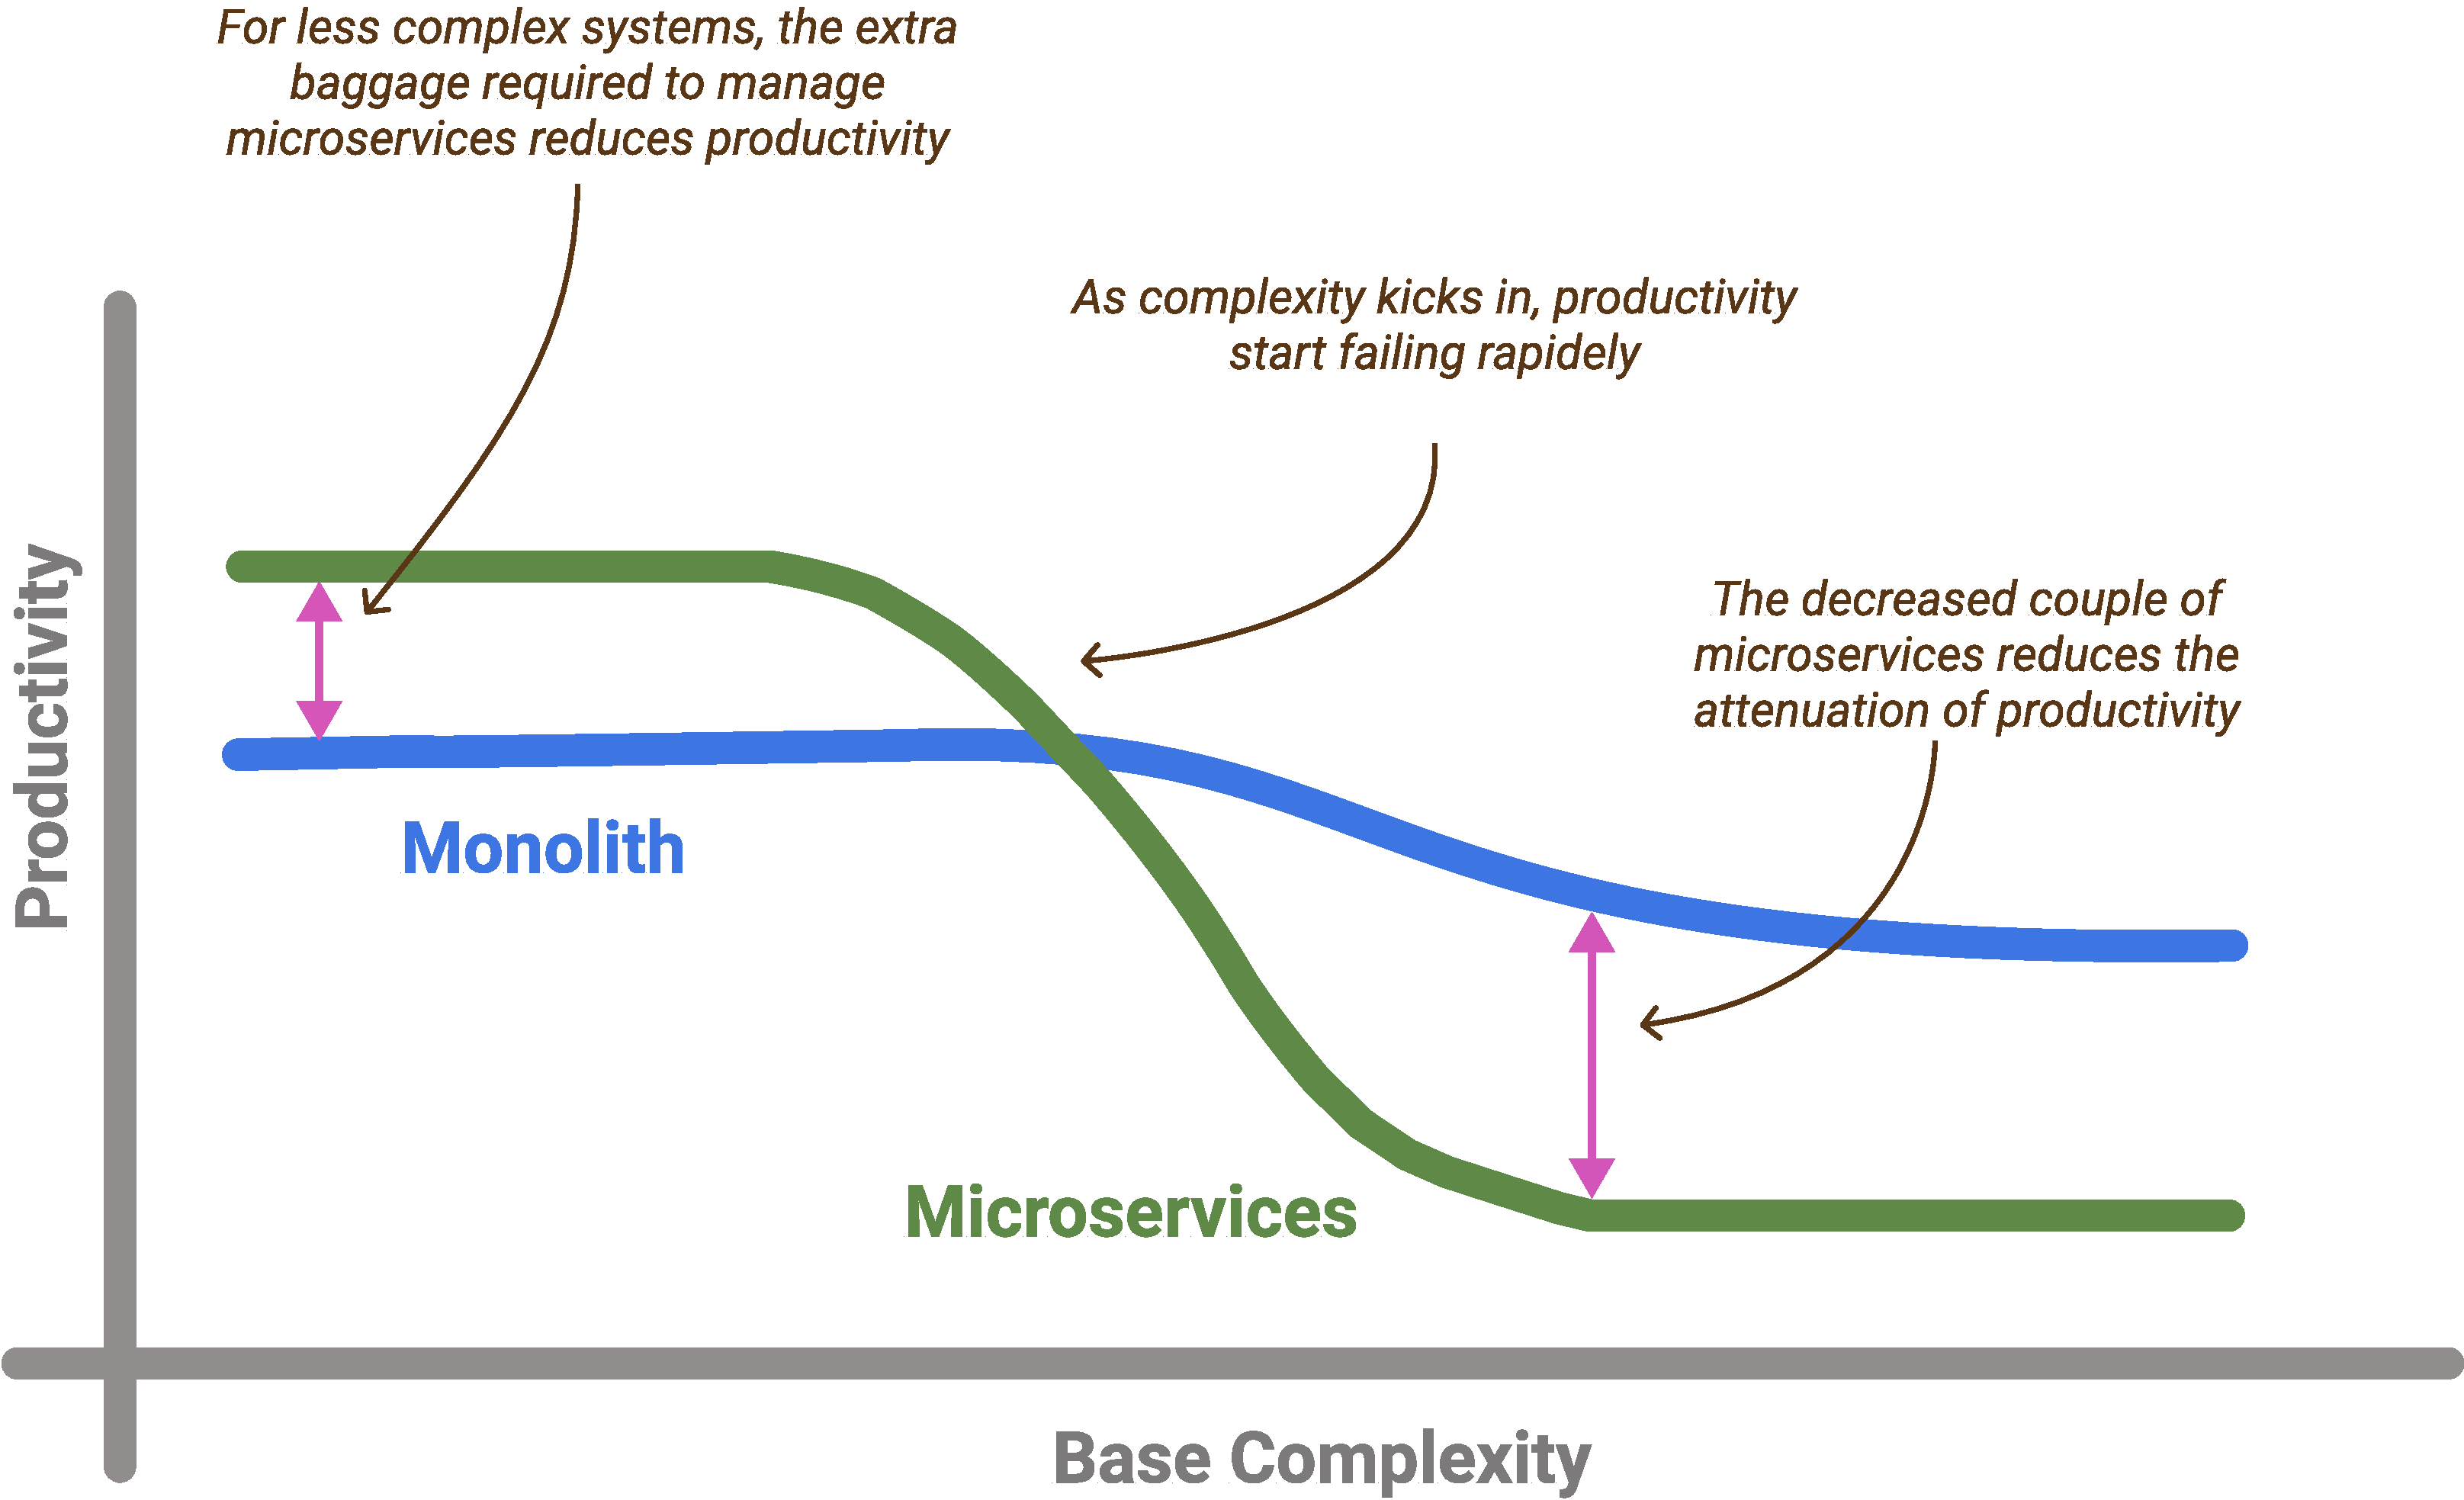
\includegraphics[width=1\textwidth]{Pictures/Monolith_vs_Microservice.pdf}
    \caption{Relation between system complexity and architectures. Source: https://martinfowler.com/bliki/MicroservicePremium.html}
    \label{fig:monolith_vs_microservice}
\end{figure}

In a logical multilayer architecture for an information system with an object-oriented design, the following four are the most common:

\begin{itemize} % source: https://en.wikipedia.org/wiki/Multitier_architecture#cite_note-5
    \item \textbf{Presentation Layer.} UI layer, view layer, presentation tier in multitier architecture.
    \item \textbf{Application Logic.} Service layer [\cite{ji2009intelligent, swetina2014toward}]
    or GRASP Controller Layer [\cite{okada2006vision}].
    \item \textbf{Business Logic.} Business logic layer, domain logic layer.
    \item \textbf{Data Access Layer.} Persistence layer, logging, networking, and other services which are required
    to support a particular business layer.
\end{itemize}

\begin{figure}[H]
    \centering
    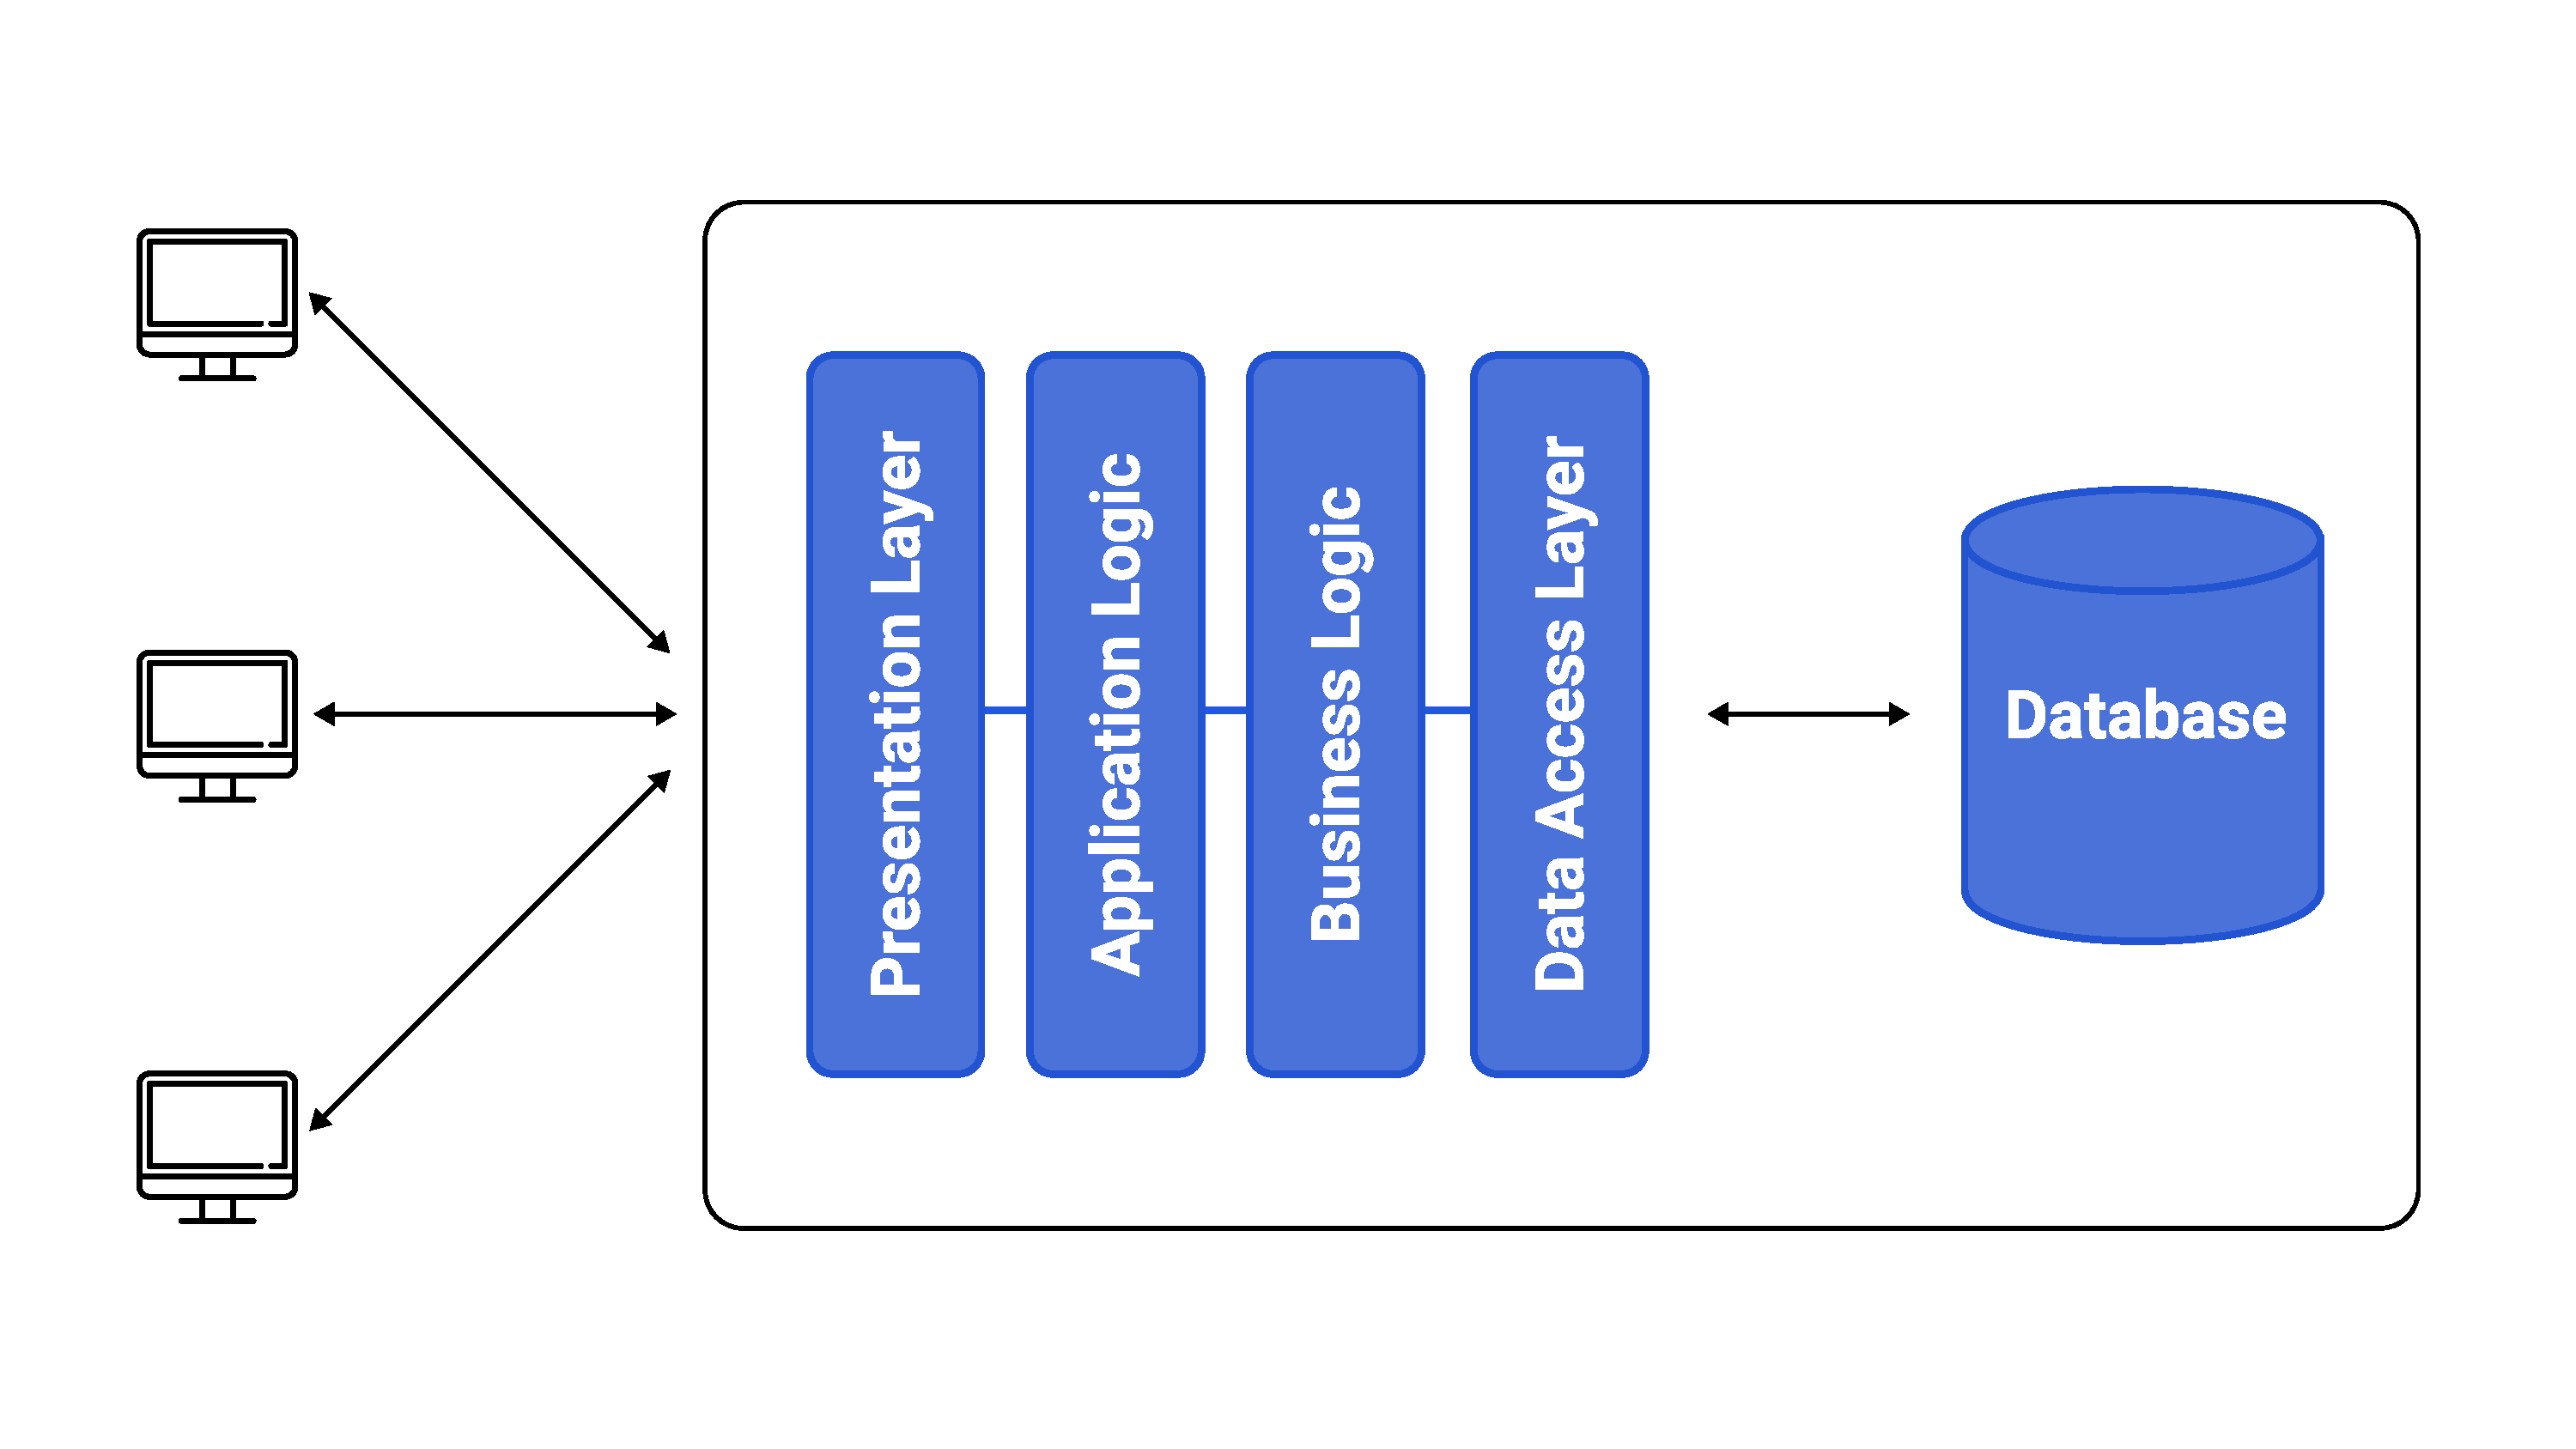
\includegraphics[width=1\textwidth]{Pictures/Monolith_architecture.pdf}
    \caption{Monolithic architecture diagram. Source: }\label{fig:figure2}
\end{figure}

The book Domain Driven Design describes some common uses for the above four layers, although its primary focus is the
domain layer [\cite{solvberg2010domain}].
If the application architecture has no explicit distinction between the business layer and the presentation layer,
then a traditional client-server model has been implemented.
The presentation layer is considered part of the business layer.
The more usual convention is that the application layer is considered a sublayer of the business layer,
typically encapsulating the API definition surfacing the supported business functionality.
The application/business layers can, in fact, be further subdivided to emphasize additional sub-layers of distinct
responsibility.
For example, if the model–view–presenter pattern is used, the presenter sublayer might be used as an additional layer
between the user interface layer and the business/application layer, as represented by the model sublayer.
Some also identify a separate layer called the business infrastructure layer, located between the business layer
and the infrastructure layer.
It's also sometimes called the \textit{low-level business layer} or the \textit{business services layer}.
The infrastructure layer can be partitioned into different levels, high-level or low-level technical services [\cite{dennis2018mcapl}].
Developers often focus on the persistence capabilities of the infrastructure layer and therefore only
talk about the persistence layer or the data access layer instead of an infrastructure layer or technical services layer.
In other words, the other kind of technical services are not always explicitly thought of as part of any particular layer.
A layer is on top of another, because it depends on it.
Every layer can exist without the layers above it, and requires the layers below it to function.
Another common view is that layers do not always strictly depend on only the adjacent layer below.
For example, in a relaxed layered system, a layer can also depend on all the layers below it [\cite{anon2014building}].
Relaxed layered system may be considered as opposed to a strict layered system.

\subsection{Monolith Architecture: Cons and Props}\label{subsec:monolith-architecture:-cons-and-props}

A monolith is built as a large system with a single code base and deployed as a single unit, usually behind a load balancer.
It typically consists of four major components: a user interface, business logic, a data interface and a database.
Monoliths offer several advantages, particularly when it comes to operational overhead requirements.
Here are some of those basic benefits:

\begin{itemize}
    \item \textbf{Simplicity.} Monolithic architectures are simple to build, test and deploy.
    These apps can scale horizontally, in one direction, by running several copies of the application behind a load balancer.
    Cross-cutting concerns: With a single codebase, monolithic apps can easily handle cross-cutting concerns, such as logging,
    configuration management and performance monitoring.
    Another advantage associated with the simplicity of monolithic apps is easier deployment.
    When it comes to monolithic applications, you do not have to handle many deployments – just one file or directory.
    \item \textbf{Performance.} Components in a monolith typically share memory which is faster than service-to-service
    communications using IPC [\cite{proctor1999linux}] or other mechanisms.
    \item \textbf{Easier debugging and testing.}
    In contrast to the microservices architecture, monolithic applications are much easier to debug and test.
    Since a monolithic app is a single indivisible unit, you can run end-to-end testing much faster.
    \item \textbf{Easier development.} As long as the monolithic approach is a standard way of building applications,
    any engineering team has the right knowledge and capabilities to develop a monolithic application.
\end{itemize}
But one major drawback of monolithic architectures is tight coupling.
Over time, monolithic components become tightly coupled and entangled.
This coupling effects management, scalability and continuous deployment.
Other cons that stem from tight coupling include:
\begin{itemize}
    \item \textbf{Understanding.} When a monolithic application scales up, it becomes too complicated to understand.
    Also, a complex system of code within one application is hard to manage.
    \item \textbf{Reliability.} An error in any of the modules in the application can bring the entire application down.
    \item \textbf{Updates.} Due to a single large codebase and tight coupling, the entire application would have to deploy
    for each update.
    \item \textbf{Technology stack.} A monolithic application must use the same technology stack throughout.
    Changes to the technology stack are expensive, both in terms of the time and cost involved.
    \item \textbf{Scalability.} You cannot scale components independently, only the whole application.
\end{itemize}

\subsection{Decoupling Monolith using CQRS}\label{subsec:decoupling-monolith-using-cqrs}
As it stated in previous section, monolithic architecture provides a quite strong coupling between application
components.
Moreover, as monolith grow horizontally, its services layer grows as well.
This process leads to very huge code base which is very difficult to support and extend.
We attach the following
\href{https://github.com/smartstore/SmartStoreNET/blob/4.x/src/Presentation/SmartStore.Web/Controllers/CatalogHelper.cs}
{link}
as an example of such approach.
To avoid the natural results of monolithic architecture, that are huge classes for thousands lines, we have to dive into
design patterns [\cite{rising1998design}].
Precisely, the mediator design pattern would help to decouple the service layer from presentation layer.
Mediator -- is a behavioral design pattern [\cite{rasche2016building}] that lets you reduce chaotic dependencies between objects.
The pattern restricts direct communications between the objects and forces them to collaborate only via a mediator object.
In other words, mediator allows the communication between two entities, such that entities doesn't know each other.
The Mediator pattern suggests that you should cease all direct communication between the components which you want to make
independent of each other.
Instead, these components must collaborate indirectly, by calling a special mediator object that redirects the calls to
appropriate components.
As a result, the components depend only on a single mediator class instead of being coupled to dozens of their colleagues.
In context of .NET platform there are multiple implementation of the Mediator, the most widely known and used is the
\href{https://github.com/jbogard/MediatR}{MediatR}, which we use in our project.
Another, yet popular approach is the CQRS, which stands for Command-Query Responsibility Segregation.
In brief, it stands that read (query) and write (command) requests should be segregated by their responsibilities.
The CQRS approach in couple with Mediator greatly helps to solve the coupling problem of the monolith architecture.
So what is CQRS precisely?
According to \href{https://martinfowler.com/bliki/CQRS.html}{Martin Fowler},
it is a pattern that first described by Greg Young [\cite{young2010cqrs}].
At its heart is the notion that you can use a different model to update information than the model you use to read information.
For some situations, this separation can be valuable, but beware that for most systems CQRS adds risky complexity.
The mainstream approach people use for interacting with an information system is to treat it as a CRUD datastore.
By this meant that we have mental model of some record structure where we can create new records, read records,
update existing records, and delete records when we're done with them.
In the simplest case, our interactions are all about storing and retrieving these records.
As our needs become more sophisticated we steadily move away from that model.
We may want to look at the information in a different way to the record store, perhaps collapsing multiple records into one,
or forming virtual records by combining information for different places.
On the update side we may find validation rules that only allow certain combinations of data to be stored, or may even infer
data to be stored that's different from that we provide.
For instance, the idea of command-query segregation is displayed at the following image

\begin{figure}[H]
    \centering
    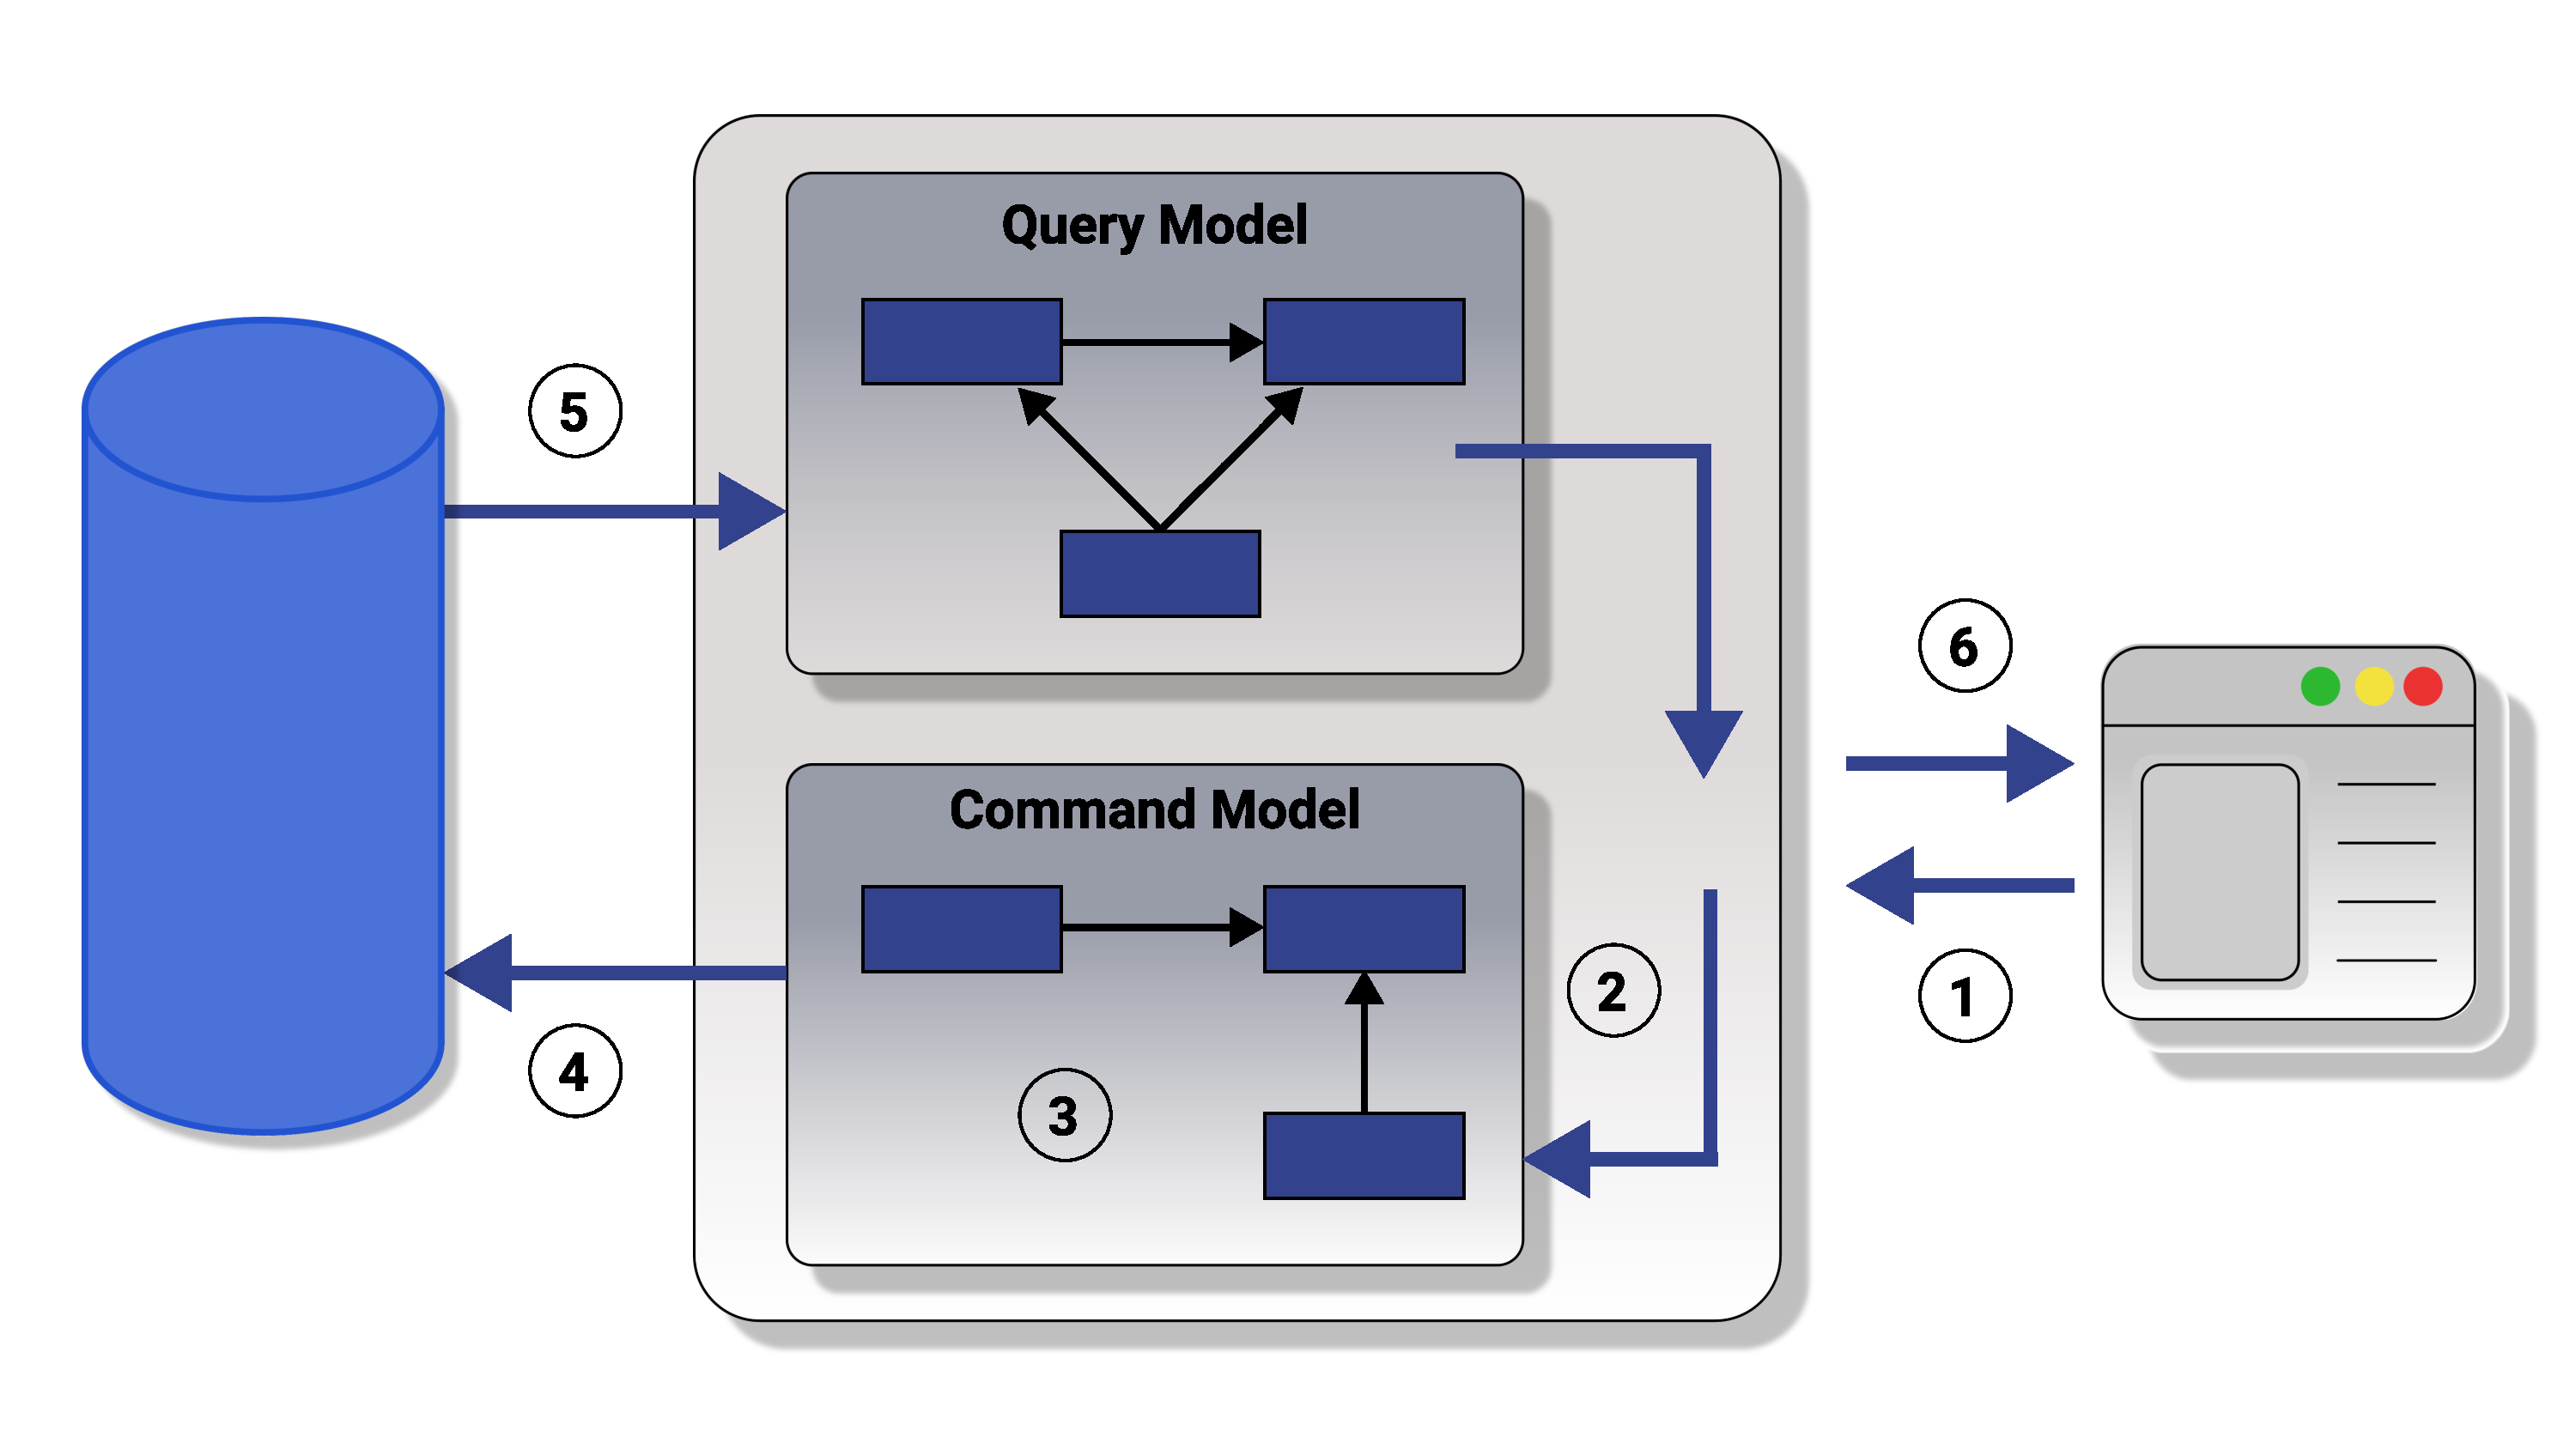
\includegraphics[width=1\textwidth]{Pictures/cqrs.pdf}
    \caption{CQRS Conceptual diagram. Source: https://martinfowler.com/bliki/CQRS.html}\label{fig:figure}
\end{figure}

\begin{enumerate}
    \item User makes a change in UI\@.
    \item Application routes information to command model.
    \item Command model executes validation and business logic.
    \item Command model updates the database.
    \item Query model reads from database.
    \item Query service update presentation from query model.
\end{enumerate}

Despite these benefits, you should be very cautious about using CQRS\@.
Many information systems fit well with the notion of an information base that is updated in the same way that it's read,
adding CQRS to such a system can add significant complexity.
I've certainly seen cases where it's made a significant drag on productivity, adding an unwarranted amount of risk to the
project, even in the hands of a capable team.
So while CQRS is a pattern that's good to have in the toolbox, beware that it is difficult to use well and you can easily
chop off important bits if you mishandle it.

As a short conclusion, we may state that CQRS and Mediator pattern will not entirely solve the coupling problems the monolith,
however will make project much more simplistic and intuitively understood.
It is worth to keep is simple,
even relatively simple project may grow to the sizes of universe without proper architectural solutions.

\subsection{Database Structure and related comments}\label{subsec:database-structure-and-related-comments}
As a next topic to uncover goes the one related to the database structure.
Proper database structure is to be of very high priority, since it influences on the project as a whole,
starting from performance point of view and many other aspects.
When we say performance, we mean such a design of database that there is an opportunity to include required indexes,
depending on regularity of any particular request.
So, as the main topic of current thesis is implementation of Instant messaging system, we can list the following
general entities to be added to database schema.

\begin{itemize}
    \item \textbf{Users.} Table stores information about user.
    Table contains following columns:
    \begin{itemize}
        \item Id VARCHAR(36) -- Id of the user, primary key, GUID\@.
        \item UserName VARCHAR(50) -- Unique Username.
        \item NormalizedUserName VARCHAR(50) -- Unique Username in upper case.
        \item DisplayName VARCHAR(50) -- Name of the user, displayed to others.
        \item Bio VARCHAR(250) -- User's short biography, visible to others.
        \item Image VARCHAR(36) -- User's profile picture, visible to others.
        \item Email VARCHAR(120) -- User's email address, not public.
        \item EmailConfirmed BOOLEAN -- Flag that indicates if user has confirmed his email address.
        \item PhoneNumber VARCHAR(50) -- User's phone number.
        \item PhoneNumberConfirmed BOOLEAN -- Flag that indicates if user has confirmed his phone number.
        \item PhoneVerificationCode INTEGER -- Code sent to user in order to confirm phone number.
        \item PasswordHash VARCHAR(60) -- Hashed password.
        \item CreatedAt DATETIME -- Indicates the date and time user has been registered.
        \item UpdatedAt DATETIME -- Indicates the date and time user has updated his record.
    \end{itemize}
    \item \textbf{User Personal Information.} Table stores additional but not required info about user.
    Relation one-to-one with Users, foreign key is UserId, GUID\@.
    Table contains following columns:
    \begin{itemize}
        \item UserId VARCHAR(36) -- Foreign key to the Users table, GUID\@.
        \item FirstName VARCHAR(120) -- First name of user.
        \item LastName VARCHAR(120) -- Last name of user.
        \item BirthDay DATETIME -- Birth day of user.
        \item WebSite VARCHAR(120) -- Web site of user.
        \item Address VARCHAR(120) -- Residence address of user.
        \item Facebook VARCHAR(120) -- Facebook nickname of user.
        \item Twitter VARCHAR(120) -- Twitter nickname of user.
        \item Instagram VARCHAR(120) -- Instagram nickname of user.
        \item LinkedIn VARCHAR(120) -- LinkedIn nickname of user.
        \item ProfilePicture VARCHAR(36) -- Avatar of user.
    \end{itemize}
    \item \textbf{UserContacts.} Table stores the contacts of current user.
    Relation between tables Users and UserContacts is one-to-many, foreign key UserId.
    Table contains following columns:
    \begin{itemize}
        \item ContactId VARCHAR(36) -- Id of current user's contact, GUID\@.
        \item UserId VARCHAR(36) -- Id of current user, GUID\@.
    \end{itemize}
    \item \textbf{Chats.} In order to communicate with other people it is essentially to have a chat room.
    Our implementation provides chat rooms of the four types.
    Direct chat -- chat room between only two members.
    Public channel -- chat room for multiple members, each member can send and read messages.\ It displayed in search results.
    Readonly channel -- channel for multiple members, however only the owner can send messages.\ It displayed in search results.
    Private channel -- channel for multiple members, can be joined only by invite link.
    Each user can have a numerous various chats, however, each chat has a multiple members, at least 2 as the case of direct chat.
    Therefore, we consider a many-to-many relation between user and chats via intermediate table UserChats.
    We discuss UserChats relation in foregoing part.
    Continuing with Chats table, it contains the following columns:
    \begin{itemize}
        \item Id VARCHAR(36) -- Id of the chat, primary key, GUID.
        \item ChatInfoId VARCHAR(36) -- Since we have a four types of channels, which has a common subset of data,
        the different data is moved to another table, so it could be joined depending on chat type.
        For instance, any chat type except direct one would require to join additional data in order to display the chat properly.
        \item Title VARCHAR(50) -- Simply, the title of the chat.
        \item Image VARCHAR(36) -- Picture of the chat.\ Displayed in search results etc.
        \item ChatType ENUM -- The type of the chat, e.g direct chat, public channel, readonly channel, private channel.
        \item CreatedAt DATETIME -- Indicates the date and time chat has been created.
        \item UpdatedAt DATETIME -- Indicates the date and time chat has been updated.
    \end{itemize}
    \item \textbf{UserChats.} Table that considered as composite key of the many-to-many relation between Users and Chats tables.
    Over that, contains an enum value that indicates user's role in the chat.
    We assume the following user roles in the system:
    \begin{itemize}
        \item Owner -- the creator of the chat.
        Has an ultimate privileges.
        \item Administrator -- designated by the owner user, which has adjustable privileges.
        \item Moderator -- designated by administrator user, which has adjustable privileges.
        \item User -- default role assigned to the user on join the chat.
    \end{itemize}
    Despite that, the UserChats table contains the following columns:
    \begin{itemize}
        \item ChatId VARCHAR(36) -- Foreign key to the Chats table, GUID\@.
        \item UserId VARCHAR(36) -- Foreign key to the Users table, GUID\@.
        \item RoleId ENUM -- Indicates the user role in the chat, e.g Owner, Administrator, Moderator, User.
    \end{itemize}
    \item \textbf{Chat Info.} Table contains additional data related to the chat.
    This table is created since that we have four types of chats, namely, direct chat, public channel,
    readonly channel, private channel.
    These four types has a common data between each other.
    Common data between chat types is Chats table itself.
    One would advise to store the chats in a single table per chat type, however it is very costly approach, since there
    would be at least four joins per request.
    Note that every chat type except direct chat requires an additional data to be displayed, that is Chat Info.
    Contains following columns:
    \begin{itemize}
        \item Id VARCHAR(36) -- Id of the chat information, primary key, GUID\@.
        \item Description VARCHAR(120) -- Description of the chat.
        \item Tag VARCHAR(20) -- Unique identifier of the chat.
        \item MembersCount INTEGER -- Count of members in the chat.
    \end{itemize}
    \item \textbf{Messages.} Table that keeps messages and related data.
    Each chat has a multiple messages, however one message must belong only to single and defined chat,
    therefore relation between Chats and Messages is one-to-many, foreign key ChatId.
    From other side, each User has a multiple messages, however single message should belong to single author,
    therefore, we consider one-to-mane relation between Users and Messages, foreign key UserId.
    Messages table contains following columns:
    \begin{itemize}
        \item Id VARCHAR(36) -- Id of the message, primary key, GUID\@.
        \item ChatId VARCHAR(36) -- Foreign key to the Chats table, GUID\@.
        \item UserId VARCHAR(36) -- Foreign key to the Users table, GUID\@.
        \item Content VARCHAR(300) -- Content of the message.
        \item IsRead BOOLEAN -- Indicates whenever message has been read by another user.
        \item CreateAt DATETIME -- Time when the message has been created.
        \item UpdatedAt DATETIME -- Time when the message has been updated.
    \end{itemize}
    \item \textbf{Refresh Tokens.} Table stores refresh tokens.
    \begin{itemize}
        \item Id VARCHAR(36) -- Id of the token, primary key, GUID\@.
        \item UserId VARCHAR(39) -- Foreign key to the Users table, GUID\@.
        \item RefreshToken VARCHAR(60) -- Refresh token itself.
        \item Expires DATETIME -- Expiration date of refresh token.
        \item CreatedAt DATETIME -- Date when token has been created.
    \end{itemize}
\end{itemize}
Following diagram demonstrates the database structure.
\begin{figure}[H]
    \centering
    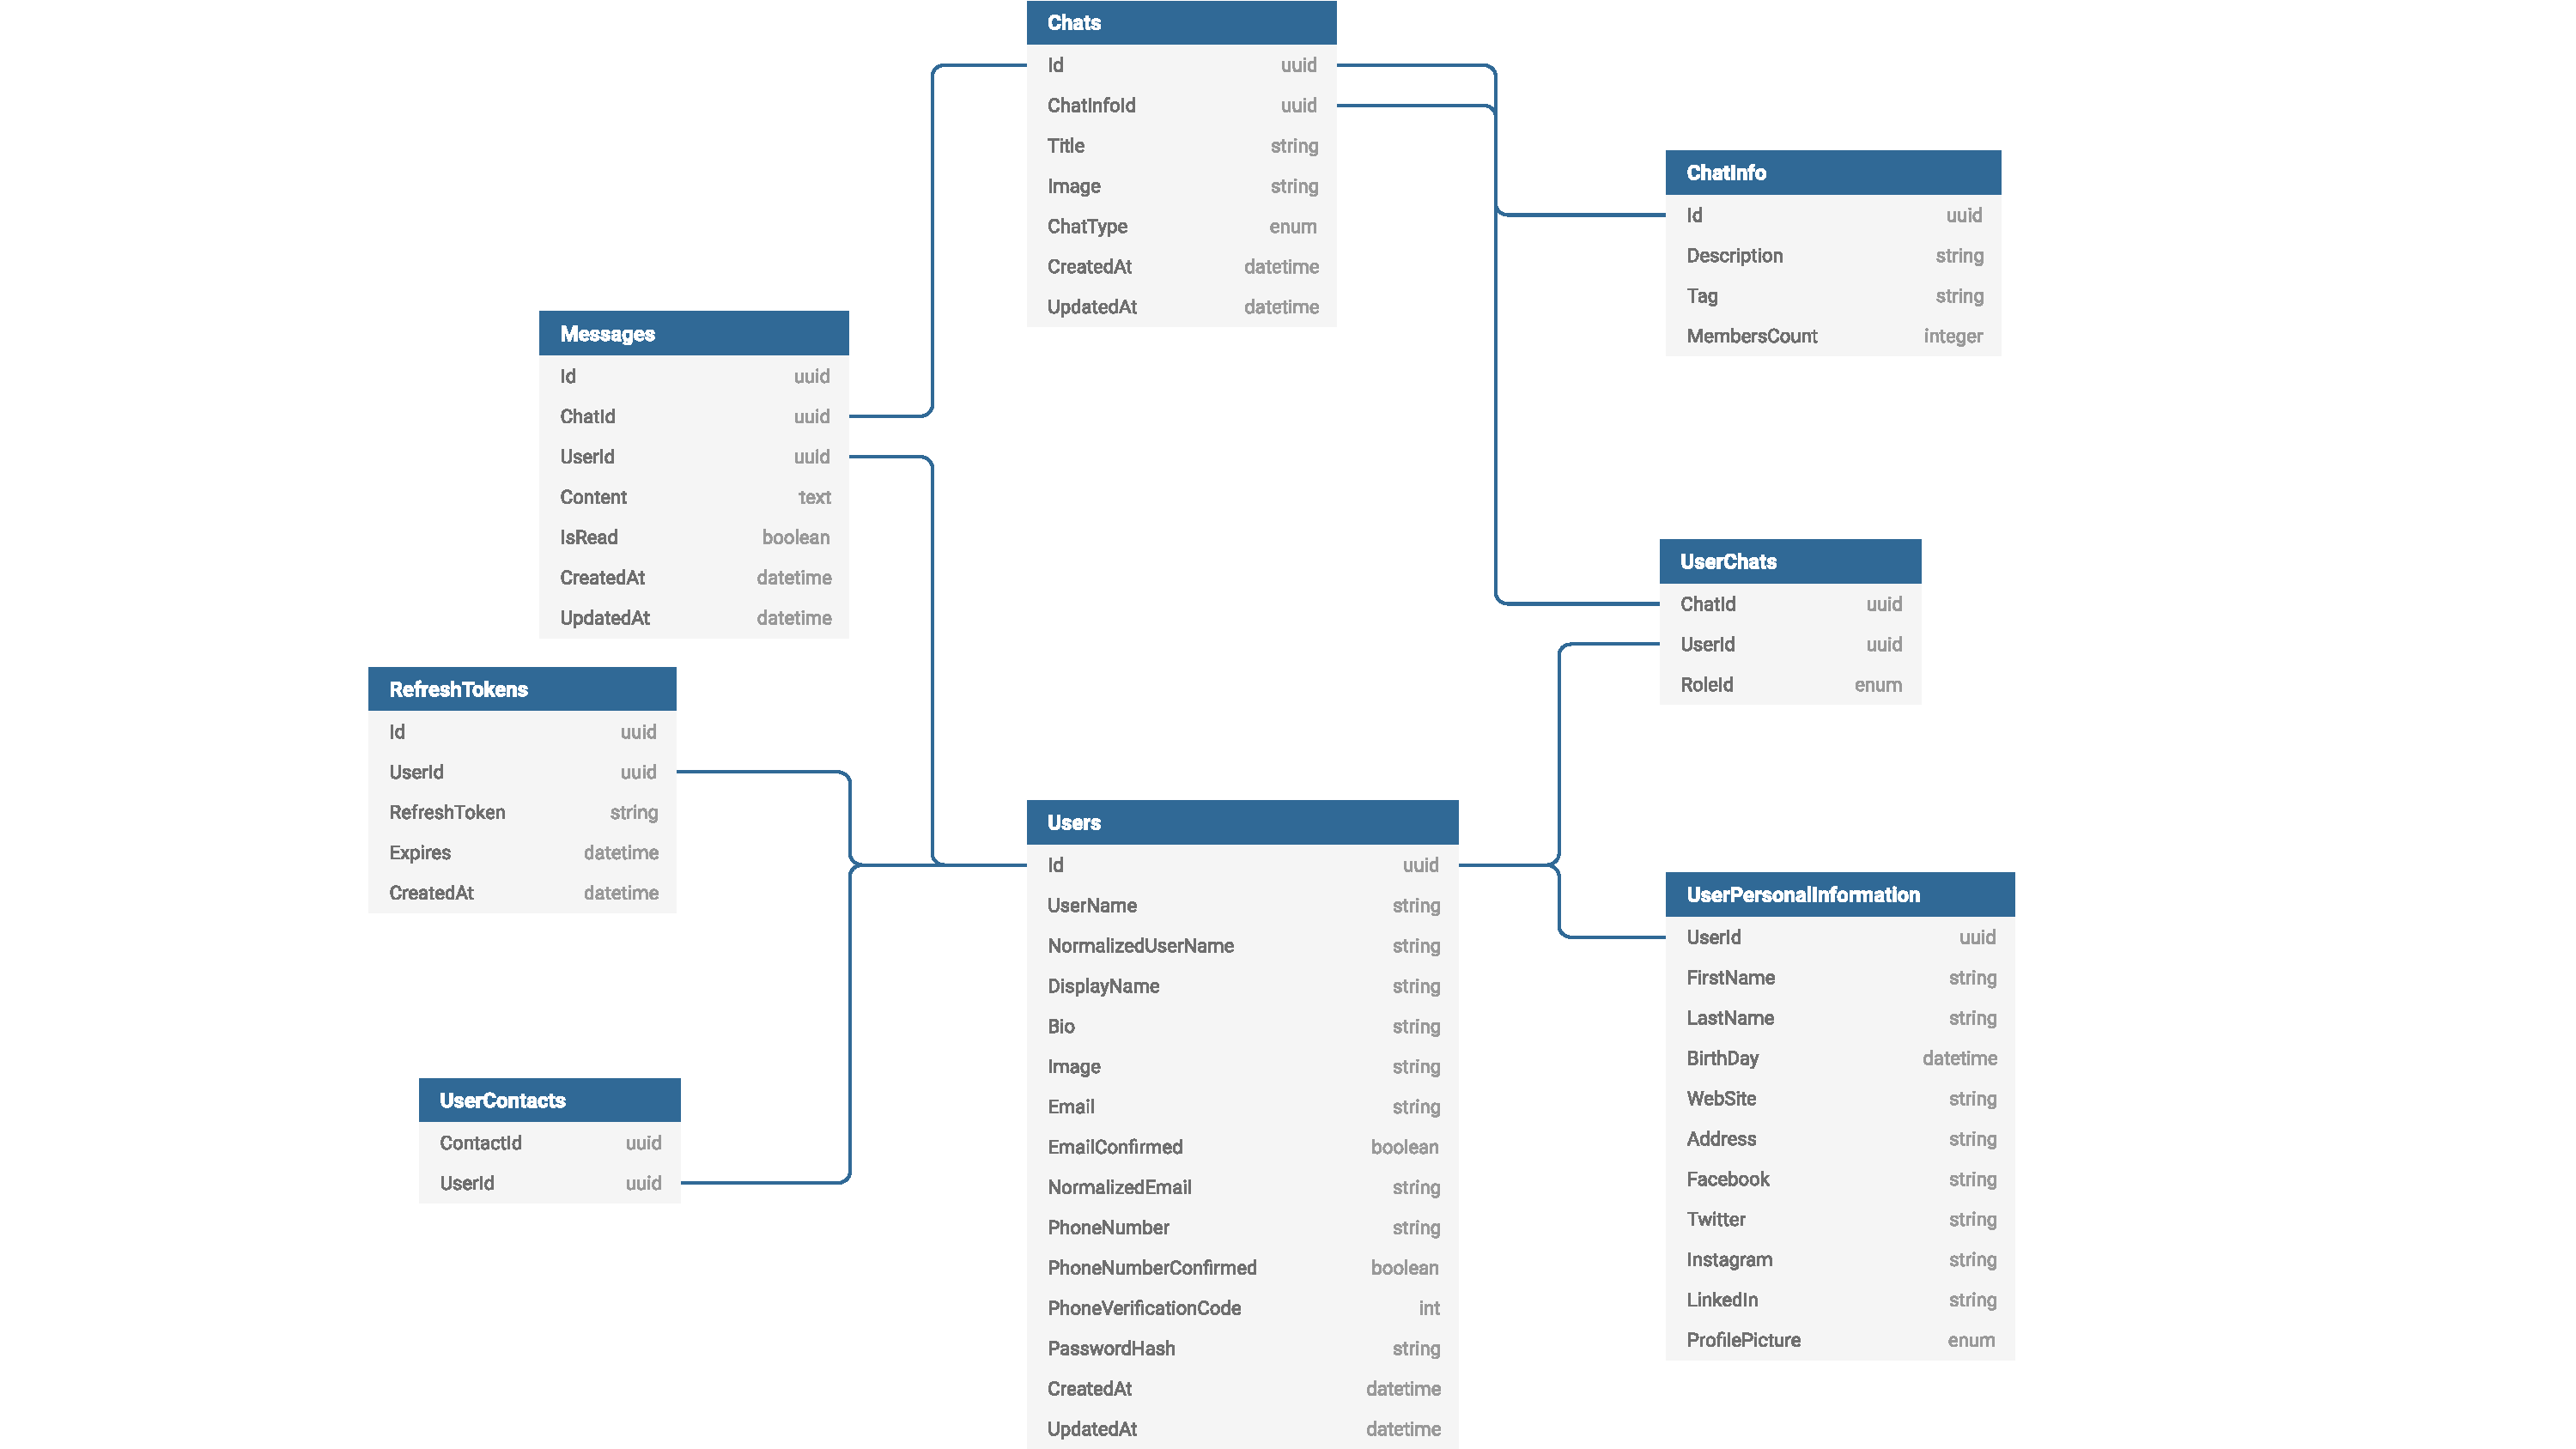
\includegraphics[width=1.2\textwidth]{Pictures/DB_diagram}
    \caption{Database diagram}\label{fig:figure5}
\end{figure}
Over whole data entities, we prefer to use universally unique identifier (UUID) or namely globally unique identifier (GUID),
a 128-bit label used for information in computer systems [\cite{leach2005universally}].
Simply, because it does not force us to keep a sequence on database side.
Sequence -- is a special entity provided in PostgreSQL relational databases.
It is responsible for generating unique values and sometimes causes a problems during migration of the database.
But still, are GUID identifiers are really always unique?
Well, each generated GUID is not guaranteed to be unique, the total number of unique keys $2^{128}$ or $3.4 \times 10^{38}$
is so large that the probability of the same number being generated twice is very small.
For example, consider the observable universe, which contains about $5 \times 10^{22}$ stars.
Every star could then have $6.8 \times 10^{15}$ universally unique GUIDs.
If you are scared of the same GUID values then put two of them next to each other.
If you are too paranoid then put three [\cite{GUIDSo}].


    \section{Motivation}\label{sec:motivation}
In this section we describe the processes of Authentication and Authorization in the system.
It is worth to remember the meaning of Authentication and Authorization definitions.
Authentication -- is the process of ascertaining that somebody really is who they claim to be [\cite{burrows1989logic}].
Authorization refers to rules that determine who is allowed to do what [\cite{fagin1978authorization}].
For example, Adam may be authorized to create and delete databases, while Eve is only authorized to read.
The two concepts are completely orthogonal and independent, but both are central to security design, and the
failure to get either one correct opens up the avenue to compromise.
In terms of web apps, very crudely speaking, authentication is when you check login credentials to see if you recognize
a user as logged in, and authorization is when you look up in your access control whether you allow the user to view,
edit, delete or create content.
As to the projects concerns, we should handle multiple client applications, e.g desktop,
web, mobile etc.
Therefore, cookie authorization doesn't fit for the project, however the JWT one surely passes.


\section{JWT Tokens}\label{sec:jwt-tokens}
So, what is JSON Web Token (JWT)?
JSON Web Token (JWT) is an open standard (RFC 7519) that defines a compact and self-contained way for securely
transmitting information between parties as a JSON object [\cite{jones2015json}].
This information can be verified and trusted because it is digitally signed.
JWTs can be signed using a secret (with the HMAC algorithm [\cite{wang2004hmac}]) or a public/private key pair using RSA or ECDSA\@.
Although JWTs can be encrypted to also provide secrecy between parties, we will focus on signed tokens.
Signed tokens can verify the integrity of the claims contained within it, while encrypted tokens hide those claims from
other parties.
When tokens are signed using public/private key pairs, the signature also certifies that only the party holding the
private key is the one that signed it.
In its compact form, JSON Web Tokens consist of three parts separated by dots, which are:
\begin{itemize}
    \item Header -- typically consists of two parts: the type of the token, which is JWT, and the signing algorithm
    being used, such as HMAC SHA256 or RSA\@.
    \item Payload -- The second part of the token is the payload, which contains the claims.
    Claims are statements about an entity (typically, the user) and additional data.
    There are three types of claims: registered, public, and private claims.
    \item Signature -- To create the signature part you have to take the encoded header, the encoded payload, a secret,
    the algorithm specified in the header, and sign that.
\end{itemize}
Therefore, a JWT typically looks like \texttt{xxxxx.yyyyy.zzzzz}.
Then, this JSON is Base64Url encoded to form the first part of the JWT\@.


\section{JWT Authentication}\label{sec:jwt-authentication}
An authentication, when the user successfully logs in using their credentials, a JSON Web Token will be returned.
Since tokens are credentials, great care must be taken to prevent security issues.
In general, you should not keep tokens longer than required.
You also should not store sensitive session data in browser storage due to lack of security.
Whenever the user wants to access a protected route or resource, the user agent should send the JWT,
typically in the Authorization header using the Bearer schema.
The content of the header should look like \texttt{Authorization: Bearer <token>}.
This can be, in certain cases, a stateless authorization mechanism.
The server's protected routes will check for a valid JWT in the Authorization header, and if it's present, the user
will be allowed to access protected resources.
If the JWT contains the necessary data, the need to query the database for certain operations may be reduced, though
this may not always be the case.
If the token is sent in the Authorization header, Cross-Origin Resource Sharing (CORS) won't be an issue as it doesn't
use cookies.
The following diagram shows how a JWT is obtained and used to access APIs or resources:
\begin{figure}[H]
    \centering
    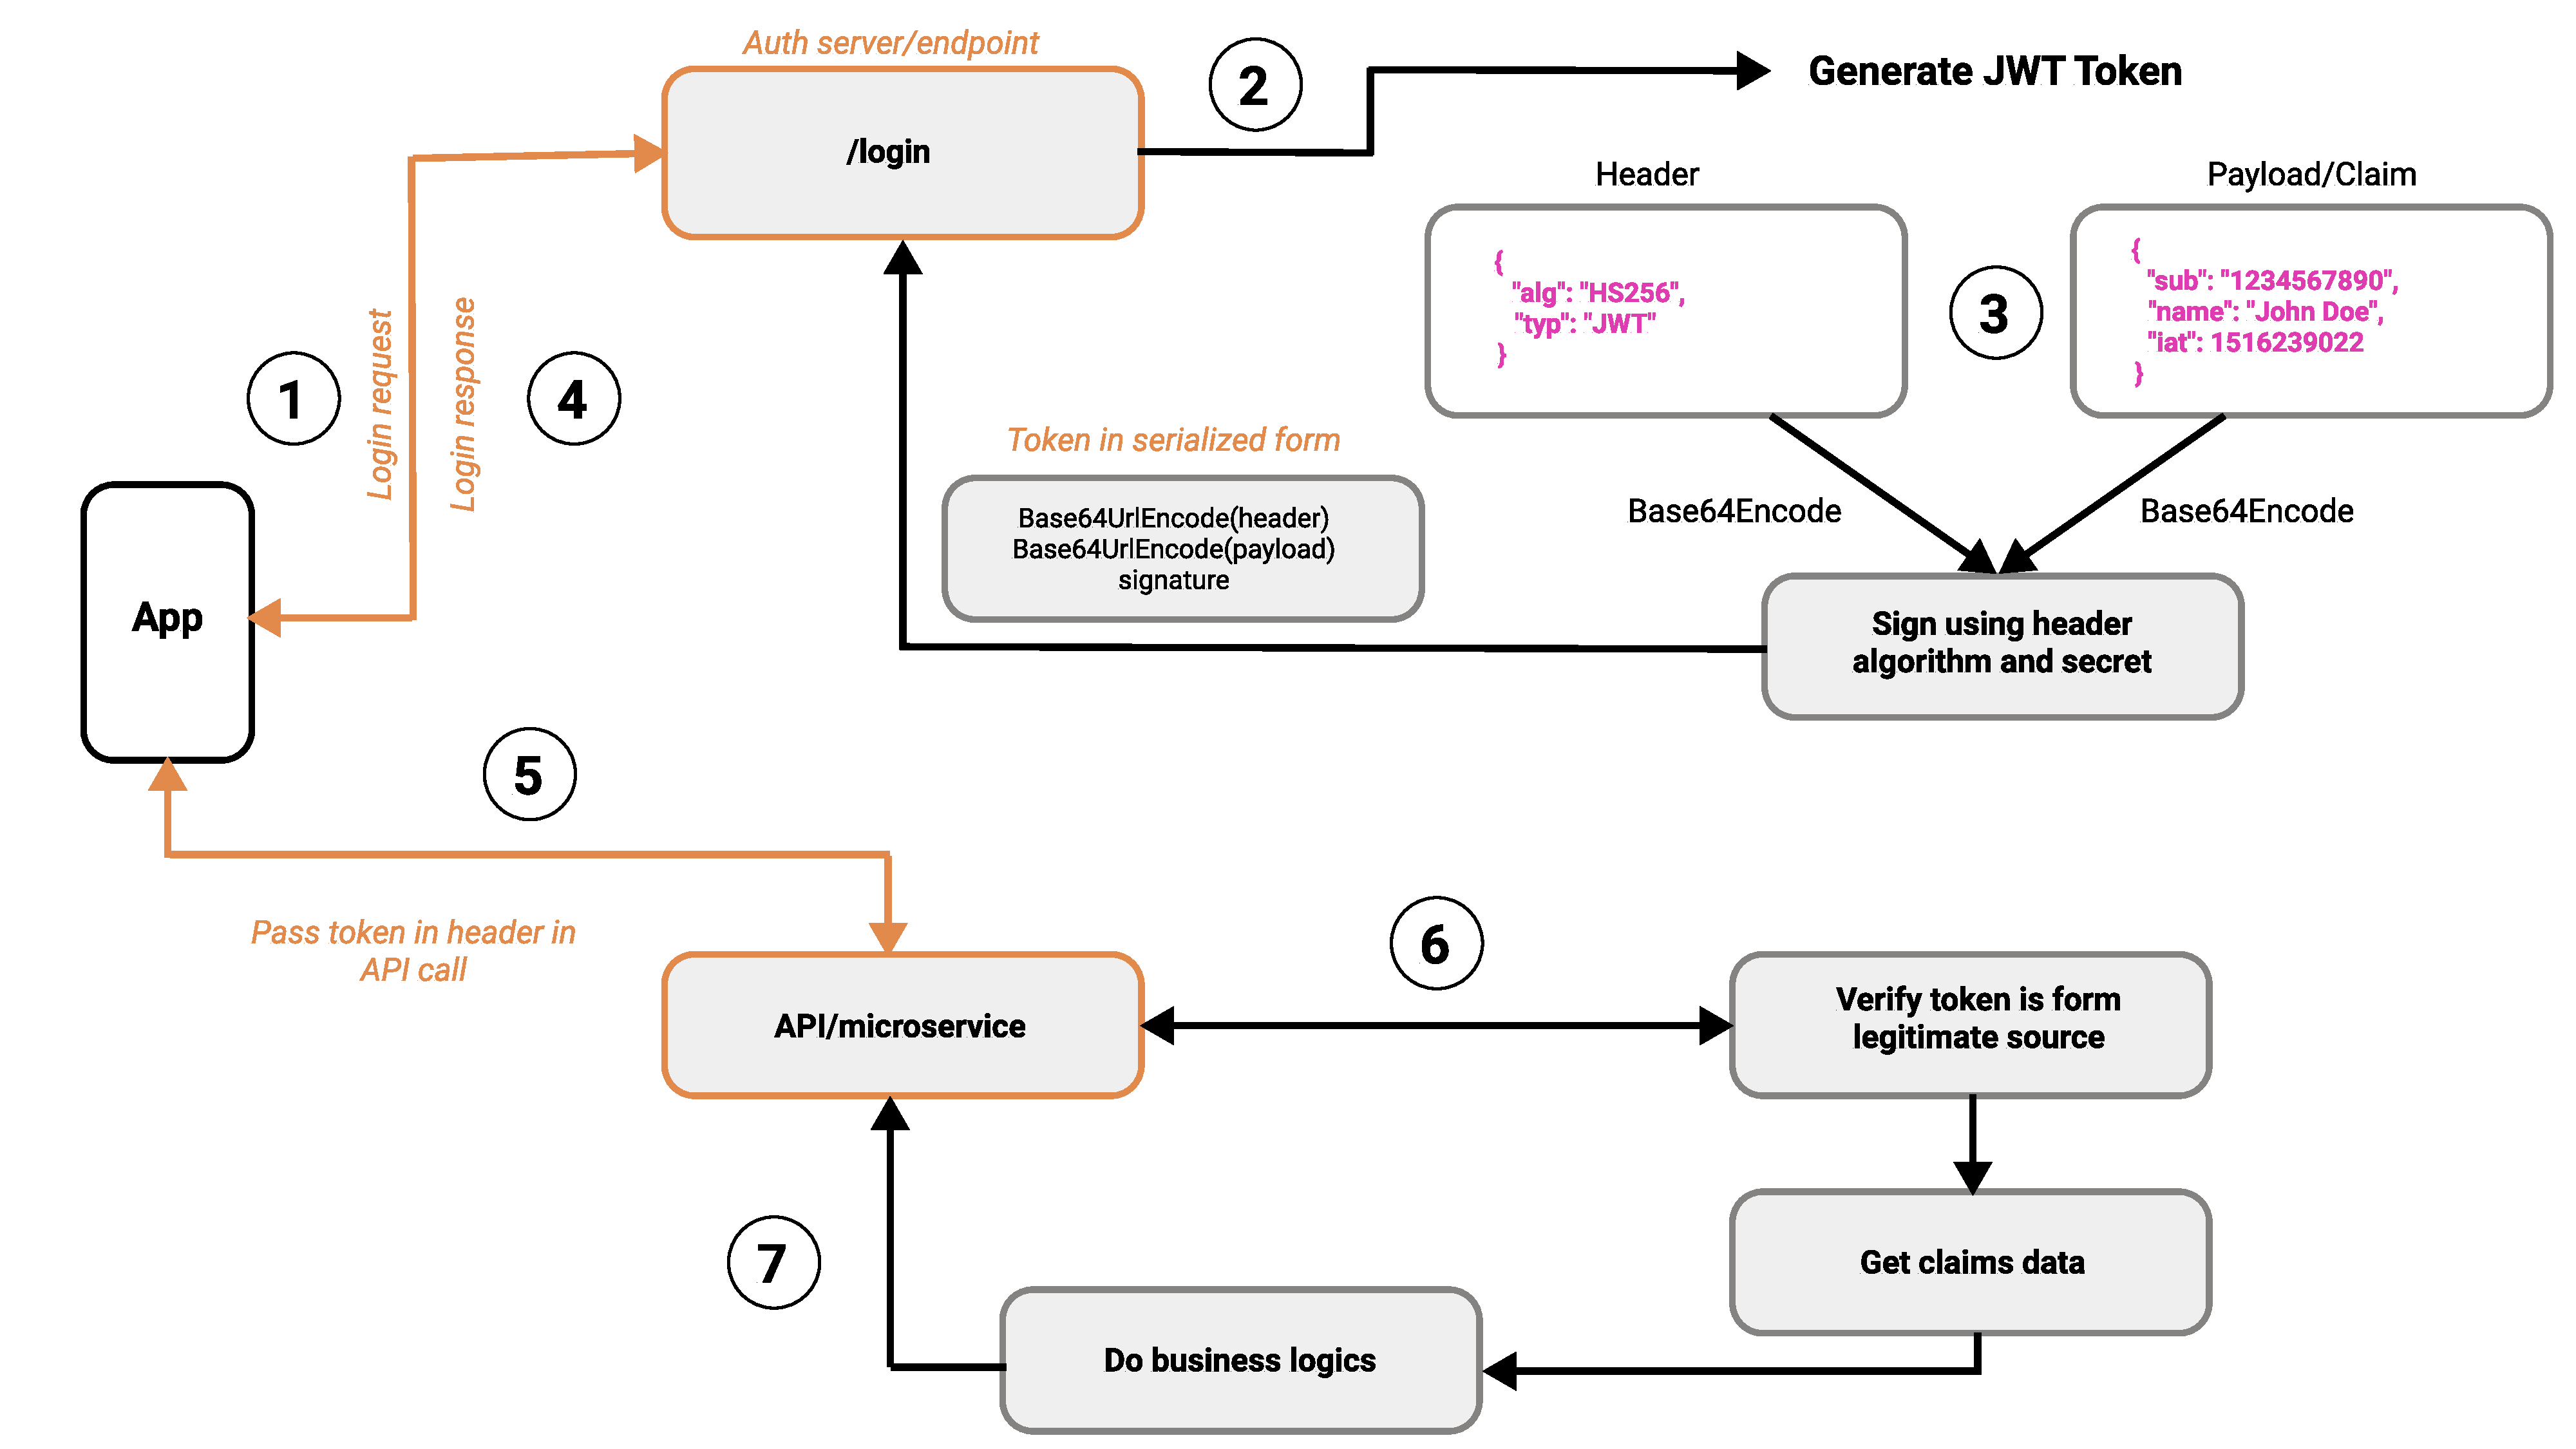
\includegraphics[width=1\textwidth]{Pictures/jwt_auth_scheme.pdf}
    \caption{JWT Authentication principle diagram.}\label{fig:figure3}
\end{figure}
JWT is quite simple and straightforward way to authorize particular person to the system's part.
However, what is about security, does it provide enough level of security?
Not really is.
When the JWT token is stolen, there is no way to revoke it.
Only the thing is to wait while token expires by himself, after its predefined lifetime.
A few basic rules about JWT usage [\cite{RDegges}]
\begin{itemize}
    \item JWT should have a short lifetime (few seconds).
    \item JWT should be used in a single time, e.g JWT per request.
\end{itemize}

%----------------------------------------------------------------------------------------
%	BIBLIOGRAPHY
%----------------------------------------------------------------------------------------

    \printbibliography[heading=bibintoc]

%----------------------------------------------------------------------------------------

    %----------------------------------------------------------------------------------------
%	THESIS CONTENT - APPENDICES
%----------------------------------------------------------------------------------------

    \appendix % Cue to tell LaTeX that the following "chapters" are Appendices

% Include the appendices of the thesis as separate files from the Appendices folder
% Uncomment the lines as you write the Appendices

    \chapter{Web API Documentation}\label{ch:web-api-documentation}


\section{Auth}\label{sec:auth}
\begin{itemize}
    %% Register Endpoint
    \item \textbf{Endpoint}: /api/auth/register
    \begin{itemize}
        \item \textbf{Description}: Registers user in a messenger
        \item \textbf{Request type}: POST
        \item \textbf{Request body}:
        \begin{spverbatim}
        {
            "phoneNumber": "string",
            "email": "string",
            "displayName": "string",
            "password": "string",
            "verificationMethod": number,
            "termsAccepted": boolean
        }
        \end{spverbatim}
        \item  \textbf{Response example}:
        \begin{itemize}
            \item \textbf{200 Success}:
            \begin{spverbatim}
            {
                "message": "SUCCESS",
                "success": true
            }
            \end{spverbatim}
            \item \textbf{400 Bad Request}:
            \begin{spverbatim}
            {
                "errorMessage": "string",
                "errorDetails": "string",
                "statusCode": 0,
                "success": true
            }
            \end{spverbatim}
            \item \textbf{409 Conflict}:
            \begin{spverbatim}
            {
                "errorMessage": "string",
                "errorDetails": "string",
                "statusCode": 0,
                "success": true
            }
            \end{spverbatim}
        \end{itemize}
        \item \textbf{Response messages}:
        \begin{enumerate}
            \item Success.
            \item User already registered.
            \item Weak password.
            \item Invalid email.
            \item Invalid verification method.
            \item Invalid display name.
            \item Phone occupied.
        \end{enumerate}
    \end{itemize}
    %% Register Endpoint

    %% Verify Email Endpoint
    \item \textbf{Endpoint}: api/auth/verify-email
    \begin{itemize}
        \item \textbf{Description}: Sends verification request.
        User receives confirmation link via email.
        \item \textbf{Request type}: POST
        \item \textbf{Request body}:
        \begin{spverbatim}
        {
            "email": "string",
            "userId": "string"
        }
        \end{spverbatim}
        \item  \textbf{Response example}:
        \begin{itemize}
            \item \textbf{200 Success}:
            \begin{spverbatim}
            {
                "message": "SUCCESS",
                "success": true
            }
            \end{spverbatim}
            \item \textbf{400 Bad Request}:
            \begin{spverbatim}
            {
                "errorMessage": "string",
                "errorDetails": "string",
                "statusCode": 0,
                "success": true
            }
            \end{spverbatim}
            \item \textbf{409 Conflict}:
            \begin{spverbatim}
            {
                "errorMessage": "string",
                "errorDetails": "string",
                "statusCode": 0,
                "success": true
            }
            \end{spverbatim}
        \end{itemize}
        \item \textbf{Response messages}:
        \begin{enumerate}
            \item Success.
            \item User already registered.
            \item Weak password.
            \item Invalid email.
            \item Invalid verification method.
            \item Invalid display name.
            \item Phone occupied.
        \end{enumerate}
        \item \textbf{Response messages}:
        \begin{enumerate}
            \item Success.
            \item Invalid user id.
            \item Email already verified.
        \end{enumerate}
    \end{itemize}
    %% Verify Email Endpoint

    %% Verify Phone Endpoint
    \item \textbf{Endpoint}: api/auth/verify-phone
    \begin{itemize}
        \item \textbf{Description}: Sends SMS to user phone.
        \item \textbf{Request type}: POST
        \item \textbf{Request body}:
        \begin{spverbatim}
        {
            "confirmationCode": 0,
            "userId": "string"
        }
        \end{spverbatim}
        \item  \textbf{Response example}:
        \begin{itemize}
            \item \textbf{200 Success}:
            \begin{spverbatim}
            {
                "message": "SUCCESS",
                "success": true
            }
            \end{spverbatim}
            \item \textbf{400 Bad Request}:
            \begin{spverbatim}
            {
                "errorMessage": "string",
                "errorDetails": "string",
                "statusCode": 0,
                "success": true
            }
            \end{spverbatim}
            \item \textbf{409 Conflict}:
            \begin{spverbatim}
            {
                "errorMessage": "string",
                "errorDetails": "string",
                "statusCode": 0,
                "success": true
            }
            \end{spverbatim}
        \end{itemize}
        \item \textbf{Response messages}:
        \begin{enumerate}
            \item Success.
            \item Invalid or expired.
            \item Phone already verified
        \end{enumerate}
    \end{itemize}
    %% Verify Phone Endpoint

    %% Login Endpoint
    \item \textbf{Endpoint}: api/auth/login
    \begin{itemize}
        \item \textbf{Description}: Performs login to the messenger.
        \item \textbf{Request type}: POST
        \item \textbf{Request body}:
        \begin{spverbatim}
        {
            "email": "string",
            "password": "string"
        }
        \end{spverbatim}
        \item \textbf{Response example}:
        \begin{itemize}
            \item \textbf{200 Success}:
            \begin{spverbatim}
            {
                "refreshTokenId": "string",
                "accessToken": "string",
                "message": "string",
                "success": true
            }
            \end{spverbatim}
            \item \textbf{400 Bad Request}:

            \begin{spverbatim}
            {
                "errorMessage": "string",
                "errorDetails": "string",
                "statusCode": 0,
                "success": true
            }
            \end{spverbatim}
            \item \textbf{409 Conflict}:
            \begin{spverbatim}
            {
                "errorMessage": "string",
                "errorDetails": "string",
                "statusCode": 0,
                "success": true
            }
            \end{spverbatim}
        \end{itemize}
        \item \textbf{Response messages}:
        \begin{enumerate}
            \item Success.
            \item Invalid credentials.
        \end{enumerate}
    \end{itemize}
    %% Login Endpoint


    %% Refresh Token Endpoint
    \item \textbf{Endpoint}: api/auth/refresh-token
    \begin{itemize}
        \item \textbf{Description}: Refreshes user's existing refresh token and access token.
        \item \textbf{Request type}: POST
        \item \textbf{Request body}:
        \begin{spverbatim}
        {
            "refreshTokenId": "string"
        }
        \end{spverbatim}
        \item  \textbf{Response example}:
        \begin{itemize}
            \item \textbf{200 Success}:
            \begin{spverbatim}
            {
                "refreshTokenId": "string",
                "accessToken": "string",
                "message": "string",
                "success": true
            }
            \end{spverbatim}
            \item \textbf{400 Bad Request}:
            \begin{spverbatim}
            {
                "errorMessage": "string",
                "errorDetails": "string",
                "statusCode": 0,
                "success": true
            }
            \end{spverbatim}
            \item \textbf{409 Conflict}:
            \begin{spverbatim}
            {
                "errorMessage": "string",
                "errorDetails": "string",
                "statusCode": 0,
                "success": true
            }
            \end{spverbatim}
        \end{itemize}
        \item \textbf{Response messages}:
        \begin{enumerate}
            \item Success.
            \item Invalid or empty refresh token.
        \end{enumerate}
    \end{itemize}
    %% Refresh Token Endpoint

    %% Logout Endpoint
    \item \textbf{Endpoint}: api/auth/logout
    \begin{itemize}
        \item \textbf{Description}: Logs out from current device.
        \item \textbf{Request type}: POST
        \item \textbf{Request body}:
        \begin{spverbatim}
        {
            "refreshTokenId": "string"
        }
        \end{spverbatim}
        \item \textbf{Response example}:
        \begin{itemize}
            \item \textbf{200 Success}:
            \begin{spverbatim}
            {
                "message": "SUCCESS",
                "success": true
            }
            \end{spverbatim}
            \item \textbf{400 Bad Request}:
            \begin{spverbatim}
            {
                "errorMessage": "string",
                "errorDetails": "string",
                "statusCode": 0,
                "success": true
            }
            \end{spverbatim}
            \item \textbf{409 Conflict}:
            \begin{spverbatim}
            {
                "errorMessage": "string",
                "errorDetails": "string",
                "statusCode": 0,
                "success": true
            }
            \end{spverbatim}
        \end{itemize}
        \item \textbf{Response messages}:
        \begin{enumerate}
            \item Success.
            \item User not found.
            \item Invalid or empty refresh token.
        \end{enumerate}
    \end{itemize}
    %% Logout Endpoint

    %% Logout All Endpoint
    \item \textbf{Endpoint}: api/auth/logout-all
    \begin{itemize}
        \item \textbf{Description}: Logs out from all devices.
        \item \textbf{Request type}: POST
        \item \textbf{Request body}:
        \begin{spverbatim}
        {
            "refreshTokenId": "string"
        }
        \end{spverbatim}
        \item  \textbf{Response example}:
        \begin{itemize}
            \item \textbf{200 Success}:
            \begin{spverbatim}
            {
                "message": "SUCCESS",
                "success": true
            }
            \end{spverbatim}
            \item \textbf{400 Bad Request}:
            \begin{spverbatim}
            {
                "errorMessage": "string",
                "errorDetails": "string",
                "statusCode": 0,
                "success": true
            }
            \end{spverbatim}
            \item \textbf{409 Conflict}:
            \begin{spverbatim}
            {
                "errorMessage": "string",
                "errorDetails": "string",
                "statusCode": 0,
                "success": true
            }
            \end{spverbatim}
        \end{itemize}
    \end{itemize}
    %% Logout All Endpoint

\end{itemize}


\section{Chats}\label{sec:chats}
\begin{itemize}
    %% Get Chats Endpoint
    \item \textbf{Endpoint}: api/chats
    \begin{itemize}
        \item \textbf{Description}: Returns list of all user's chats.
        \item \textbf{Request type}: GET
        \item \textbf{Response example}:
        \textbf{200 Success}:
        \begin{spverbatim}
        {
            "chats": [
                {
                "chatId": "string",
                "title": "string",
                "image": "string",
                "lastMessageAuthor": "string",
                "lastMessage": "string",
                "lastMessageAt": "string",
                "membersCount": 0,
                "isMember": true
            }
            ],
            "message": "string",
            "success": true
        }
        \end{spverbatim}
        \textbf{400 Bad Request}:
        \begin{spverbatim}
        {
            "errorMessage": "string",
            "errorDetails": "string",
            "statusCode": 0,
            "success": true
        }
        \end{spverbatim}
        \textbf{409 Conflict}:
        \begin{spverbatim}
        {
            "errorMessage": "string",
            "errorDetails": "string",
            "statusCode": 0,
            "success": true
        }
        \end{spverbatim}
        \item \textbf{Response messages}:
        \begin{enumerate}
            \item Success.
            \item User not found.
        \end{enumerate}
    \end{itemize}
    %% Get Chats Endpoint

    %% Create Group Endpoint
    \item \textbf{Endpoint}: api/chats/group
    \begin{itemize}
        \item \textbf{Description}: Creates new group of specified type.
        \item \textbf{Request type}: POST
        \item \textbf{Request body}:
        \begin{spverbatim}
        {
            "groupType": 1
            "groupTitle": "string"
        }
        \end{spverbatim}
        \item \textbf{Chat types}:
        \begin{enumerate}
            \item DirectChat -- Chat between two people
            \item PrivateChannel -- Channel that can be joined only via invite link from owner or one of the members
            \item PublicChannel -- Channel that can be joined and messaged by anyone, unless person is not in blacklist
            \item ReadOnlyChannel -- Channel that can be joined by anyone, but any member except owner or moderator cannot send messages there
        \end{enumerate}
        \item \textbf{Response example}:
        \textbf{200 Success}:
        \begin{spverbatim}
        {
            "chatId": "string",
            "message": "string",
            "success": true
        }
        \end{spverbatim}
        \textbf{400 Bad Request}:
        \begin{spverbatim}
        {
            "errorMessage": "string",
            "errorDetails": "string",
            "statusCode": 0,
            "success": true
        }
        \end{spverbatim}
        \textbf{409 Conflict}:
        \begin{spverbatim}
        {
            "errorMessage": "string",
            "errorDetails": "string",
            "statusCode": 0,
            "success": true
        }
        \end{spverbatim}
        \item \textbf{Response messages}:
        \begin{enumerate}
            \item Success.
            \item User not found.
        \end{enumerate}
    \end{itemize}
    %% Create Group Endpoint

    %% Create Direct Chat Endpoint
    \item \textbf{Endpoint}: api/chats/direct-chat
    \begin{itemize}
        \item \textbf{Description}: Creates new group of specified type.
        \item \textbf{Request type}: POST
        \item \textbf{Request body}:
        \begin{spverbatim}
        {
            "partnerId": "string"
        }
        \end{spverbatim}
        \item \textbf{Response example}:
        \textbf{200 Success}:
        \begin{spverbatim}
        {
            "chatId": "string",
            "message": "string",
            "success": true
        }
        \end{spverbatim}
        \textbf{400 Bad Request}:
        \begin{spverbatim}
        {
            "errorMessage": "string",
            "errorDetails": "string",
            "statusCode": 0,
            "success": true
        }
        \end{spverbatim}
        \textbf{409 Conflict}:
        \begin{spverbatim}
        {
            "errorMessage": "string",
            "errorDetails": "string",
            "statusCode": 0,
            "success": true
        }
        \end{spverbatim}
        \item \textbf{Response messages}:
        \begin{enumerate}
            \item Success.
            \item User not found.
        \end{enumerate}
    \end{itemize}
    %% Create Direct Chat Endpoint

    %% Group Join Endpoint
    \item \textbf{Endpoint}: api/chats/group/join/\{chatId\}
    \begin{itemize}
        \item \textbf{Description}: Creates new group of specified type.
        \item \textbf{Request type}: POST
        \item \textbf{Request example}:
        \begin{spverbatim}
        {
            "chatId": "string"
        }
        \end{spverbatim}
        \item \textbf{Response example}:
        \textbf{200 Success}:
        \begin{spverbatim}
        {
            "chatId": "string",
            "message": "string",
            "success": true
        }
        \end{spverbatim}
        \textbf{400 Bad Request}:
        \begin{spverbatim}
        {
            "errorMessage": "string",
            "errorDetails": "string",
            "statusCode": 0,
            "success": true
        }
        \end{spverbatim}
        \textbf{409 Conflict}:
        \begin{spverbatim}
        {
            "errorMessage": "string",
            "errorDetails": "string",
            "statusCode": 0,
            "success": true
        }
        \end{spverbatim}
        \item \textbf{Response messages}:
        \begin{enumerate}
            \item Success.
            \item Group not found.
        \end{enumerate}
    \end{itemize}
    %% Group Join Endpoint

    %% Search Chat Endpoint
    \item \textbf{Endpoint}: api/chats/search
    \begin{itemize}
        \item \textbf{Description}: Searches chats by display name.
        \item \textbf{Request type}: GET
        \item \textbf{Parameters}:
        \begin{enumerate}
            \item displayName (required)
        \end{enumerate}
        \item \textbf{Response example}:
        \textbf{200 Success}:
        \begin{spverbatim}
        {
            "chats": [
                {
                "chatId": "string",
                "title": "string",
                "image": "string",
                "lastMessageAuthor": "string",
                "lastMessage": "string",
                "lastMessageAt": "string",
                "membersCount": 0,
                "isMember": true
            }
            ],
            "message": "string",
            "success": true
        }
        \end{spverbatim}
        \textbf{400 Bad Request}:
        \begin{spverbatim}
        {
            "errorMessage": "string",
            "errorDetails": "string",
            "statusCode": 0,
            "success": true
        }
        \end{spverbatim}
        \textbf{409 Conflict}:
        \begin{spverbatim}
        {
            "errorMessage": "string",
            "errorDetails": "string",
            "statusCode": 0,
            "success": true
        }
        \end{spverbatim}
        \item \textbf{Response messages}:
        \begin{enumerate}
            \item Success.
            \item Unauthorized.
        \end{enumerate}
    \end{itemize}
    %% Search Chat Endpoint

\end{itemize}


\section{Messages}\label{sec:messages}
\begin{itemize}
    %% Get Chat Messages Endpoint
    \item \textbf{Endpoint}: /api/messages/\{chatId\}
    \begin{itemize}
        \item \textbf{Description}: Returns chat including messages by chat id.
        \item \textbf{Request type}: GET
        \item \textbf{Parameters}:
        \begin{enumerate}
            \item Chat id (required).
        \end{enumerate}
        \item \textbf{Response example}:
        \begin{itemize}
            \item \textbf{200 Success}:
            \begin{spverbatim}
            {
                "messages": [
                    {
                        "userDisplayName": "string",
                        "messageText": "string",
                        "sentAt": "string",
                        "editedAt": "string",
                        "self": true
                    }
                ],
                "message": "string",
                "success": true
            }
            \end{spverbatim}
            \item \textbf{400 Bad Request}:
            \begin{spverbatim}
            {
                "errorMessage": "string",
                "errorDetails": "string",
                "statusCode": 0,
                "success": true
            }
            \end{spverbatim}
            \item \textbf{409 Conflict}:
            \begin{spverbatim}
            {
                "errorMessage": "string",
                "errorDetails": "string",
                "statusCode": 0,
                "success": true
            }
            \end{spverbatim}
        \end{itemize}
        \item \textbf{Response messages}:
        \begin{enumerate}
            \item Success.
            \item User not found.
        \end{enumerate}
    \end{itemize}
    %% Get Chat Messages Endpoint

    %% Send Message Endpoint
    \item \textbf{Endpoint}: /api/messages
    \begin{itemize}
        \item \textbf{Description}: Sends message to particular chat
        \item \textbf{Request type}: POST
        \item \textbf{Request body}:
        \begin{spverbatim}
        {
            "messageId": "string",
            "message": "string",
            "success": true
        }
        \end{spverbatim}
        \item \textbf{Response example}:
        \begin{itemize}
            \item \textbf{200 Success}:
            \begin{spverbatim}
            {
                "message": "SUCCESS",
                "success": true
            }
            \end{spverbatim}
            \item \textbf{400 Bad Request}:
            \begin{spverbatim}
            {
                "errorMessage": "string",
                "errorDetails": "string",
                "statusCode": 0,
                "success": true
            }
            \end{spverbatim}
            \item \textbf{409 Conflict}:
            \begin{spverbatim}
            {
                "errorMessage": "string",
                "errorDetails": "string",
                "statusCode": 0,
                "success": true
            }
            \end{spverbatim}
        \end{itemize}
        \item \textbf{Response messages}:
        \begin{enumerate}
            \item Success.
            \item User not found.
        \end{enumerate}
    \end{itemize}
    %% Send Message Endpoint

    %% Edit Message Endpoint
    \item \textbf{Endpoint}: /api/messages
    \begin{itemize}
        \item \textbf{Description}: Updates particular message
        \item \textbf{Request type}: PUT
        \item \textbf{Request body}:
        \begin{spverbatim}
        {
            "messageId": "string",
            "modifiedText": "string"
        }
        \end{spverbatim}
        \item \textbf{Response example}:
        \begin{itemize}
            \item \textbf{200 Success}:
            \begin{spverbatim}
            {
                "message": "SUCCESS",
                "success": true
            }
            \end{spverbatim}
            \item \textbf{400 Bad Request}:
            \begin{spverbatim}
            {
                "errorMessage": "string",
                "errorDetails": "string",
                "statusCode": 0,
                "success": true
            }
            \end{spverbatim}
            \item \textbf{409 Conflict}:
            \begin{spverbatim}
            {
                "errorMessage": "string",
                "errorDetails": "string",
                "statusCode": 0,
                "success": true
            }
            \end{spverbatim}
        \end{itemize}
        \item \textbf{Response messages}:
        \begin{enumerate}
            \item Success.
            \item User not found.
        \end{enumerate}
    \end{itemize}
    %% Edit Message Endpoint

    %% Delete Message Endpoint
    \item \textbf{Endpoint}: /api/messages
    \begin{itemize}
        \item \textbf{Description}: Deletes particular message
        \item \textbf{Request type}: DELETE
        \item \textbf{Request body}:
        \begin{spverbatim}
        {
            "messageId": "string"
        }
        \end{spverbatim}
        \item \textbf{Response example}:
        \begin{itemize}
            \item \textbf{200 Success}:
            \begin{spverbatim}
            {
                "message": "SUCCESS",
                "success": true
            }
            \end{spverbatim}
            \item \textbf{400 Bad Request}:
            \begin{spverbatim}
            {
                "errorMessage": "string",
                "errorDetails": "string",
                "statusCode": 0,
                "success": true
            }
            \end{spverbatim}
            \item \textbf{409 Conflict}:
            \begin{spverbatim}
            {
                "errorMessage": "string",
                "errorDetails": "string",
                "statusCode": 0,
                "success": true
            }
            \end{spverbatim}
        \end{itemize}
        \item \textbf{Response messages}:
        \begin{enumerate}
            \item Success.
            \item User not found.
        \end{enumerate}
    \end{itemize}
    %% Delete Message Endpoint
\end{itemize}


\section{User}\label{sec:user}
\begin{itemize}
    %% Get User Endpoint
    \item \textbf{Endpoint}: /api/users/\{userId\}
    \begin{itemize}
        \item \textbf{Description}: Returns information about particular user by user ID
        \item \textbf{Request type}: GET
        \item \textbf{Parameters}:
        \begin{enumerate}
            \item User ID (required).
        \end{enumerate}
        \item \textbf{Response example}:
        \textbf{200 Success}:
        \begin{spverbatim}
        {
            "message": "string",
            "success": true
        }
        \end{spverbatim}
        \textbf{400 Bad Request}:
        \begin{spverbatim}
        {
            "errorMessage": "string",
            "errorDetails": "string",
            "statusCode": 0,
            "success": true
        }
        \end{spverbatim}
        \textbf{409 Conflict}:
        \begin{spverbatim}
        {
            "errorMessage": "string",
            "errorDetails": "string",
            "statusCode": 0,
            "success": true
        }
        \end{spverbatim}
        \item \textbf{Response messages}:
        \begin{enumerate}
            \item Success.
            \item User not found.
        \end{enumerate}
    \end{itemize}
    %% Get User Endpoint
    %% Get Current User Endpoint
    \item \textbf{Endpoint}: /api/users
    \begin{itemize}
        \item \textbf{Description}: Returns information about current user logged in system
        \item \textbf{Request type}: GET
        \item \textbf{Response example}:
        \textbf{200 Success}:
        \begin{spverbatim}
        {
            "user": {
            "username": "string",
            "displayName": "string",
            "bio": "string",
            "image": "string"
        },
            "message": "string",
            "success": true
        }
        \end{spverbatim}
        \textbf{400 Bad Request}:
        \begin{spverbatim}
        {
            "errorMessage": "string",
            "errorDetails": "string",
            "statusCode": 0,
            "success": true
        }
        \end{spverbatim}
        \textbf{409 Conflict}:
        \begin{spverbatim}
        {
            "errorMessage": "string",
            "errorDetails": "string",
            "statusCode": 0,
            "success": true
        }
        \end{spverbatim}
        \item \textbf{Response messages}:
        \begin{enumerate}
            \item Success.
            \item User not found.
        \end{enumerate}
    \end{itemize}
    %% Get Loged User Endpoint
    %% Search User Endpoint
    \item \textbf{Endpoint}: /api/users/search
    \begin{itemize}
        \item \textbf{Description}: Searches user by display name
        \item \textbf{Request type}: GET
        \item \textbf{Parameters}:
        \begin{enumerate}
            \item displayName (required)
        \end{enumerate}
        \item \textbf{Response example}:
        \textbf{200 Success}:
        \begin{spverbatim}
        {
            "user": {
            "username": "string",
            "displayName": "string",
            "bio": "string",
            "image": "string"
        },
            "message": "string",
            "success": true
        }
        \end{spverbatim}
        \textbf{400 Bad Request}:
        \begin{spverbatim}
        {
            "errorMessage": "string",
            "errorDetails": "string",
            "statusCode": 0,
            "success": true
        }
        \end{spverbatim}
        \textbf{409 Conflict}:
        \begin{spverbatim}
        {
            "errorMessage": "string",
            "errorDetails": "string",
            "statusCode": 0,
            "success": true
        }
        \end{spverbatim}
        \item \textbf{Response messages}:
        \begin{enumerate}
            \item Success.
            \item User not found.
        \end{enumerate}
    \end{itemize}
    %% Search User Endpoint
\end{itemize}


\section{Contacts}\label{sec:contacts}
\begin{itemize}
    %% Add Contact Endpoint
    \item \textbf{Endpoint}: /api/contacts
    \begin{itemize}
        \item \textbf{Description}: Adds new contact
        \item \textbf{Request type}: POST
        \item \textbf{Request body}:
        \begin{spverbatim}
        {
            "contactId": "string"
        }
        \end{spverbatim}
        \item \textbf{Response example}:
        \textbf{200 Success}:
        \begin{spverbatim}
        {
            "message": "string",
            "success": true
        }
        \end{spverbatim}
        \textbf{400 Bad Request}:
        \begin{spverbatim}
        {
            "errorMessage": "string",
            "errorDetails": "string",
            "statusCode": 0,
            "success": true
        }
        \end{spverbatim}
        \textbf{409 Conflict}:
        \begin{spverbatim}
        {
            "errorMessage": "string",
            "errorDetails": "string",
            "statusCode": 0,
            "success": true
        }
        \end{spverbatim}
        \item \textbf{Response messages}:
        \begin{enumerate}
            \item Success.
            \item User not found.
        \end{enumerate}
    \end{itemize}
    %% Add Contact Endpoint
    %% Get Contacts Endpoint
    \item \textbf{Endpoint}: /api/contacts
    \begin{itemize}
        \item \textbf{Description}: Returns list of all user's contacts
        \item \textbf{Request type}: GET
        \item \textbf{Response example}:
        \textbf{200 Success}:
        \begin{spverbatim}
        {
            "contacts": [
                {
                "username": "string",
                "displayName": "string",
                "bio": "string",
                "image": "string"
            }
            ],
            "message": "string",
            "success": true
        }
        \end{spverbatim}
        \textbf{400 Bad Request}:
        \begin{spverbatim}
        {
            "errorMessage": "string",
            "errorDetails": "string",
            "statusCode": 0,
            "success": true
        }
        \end{spverbatim}
        \textbf{409 Conflict}:
        \begin{spverbatim}
        {
            "errorMessage": "string",
            "errorDetails": "string",
            "statusCode": 0,
            "success": true
        }
        \end{spverbatim}
        \item \textbf{Response messages}:
        \begin{enumerate}
            \item Success.
            \item User not found.
        \end{enumerate}
    \end{itemize}
    %% Get Contacts Endpoint
\end{itemize}


\section{User Information}\label{sec:user-information}
\begin{itemize}
    %% Update User Info Endpoint
    \item \textbf{Endpoint}: /api/contacts
    \begin{itemize}
        \item \textbf{Description}: Updates current user information
        \item \textbf{Request type}: PUT
        \item \textbf{Request body}:
        \begin{spverbatim}
        {
            "firstName": "string",
            "lastName": "string",
            "birthDay": "timestamp",
            "website": "string",
            "address": "string",
            "facebook": "string",
            "twitter": "string",
            "instagram": "string",
            "linkedIn": "string",
            "profilePicture": "string"
        }
        \end{spverbatim}
        \item \textbf{Response example}:
        \begin{itemize}
            \item \textbf{200 Success}:
            \begin{spverbatim}
            {
                "message": "string",
                "success": true
            }
            \end{spverbatim}
            \item \textbf{400 Bad Request}:
            \begin{spverbatim}
            {
                "errorMessage": "string",
                "errorDetails": "string",
                "statusCode": 0,
                "success": true
            }
            \end{spverbatim}
            \item \textbf{409 Conflict}:
            \begin{spverbatim}
            {
                "errorMessage": "string",
                "errorDetails": "string",
                "statusCode": 0,
                "success": true
            }
            \end{spverbatim}
        \end{itemize}
        \item \textbf{Response messages}:
        \begin{enumerate}
            \item Success.
            \item User not found.
        \end{enumerate}
    \end{itemize}
    %% Update User Info Endpoint
\end{itemize}
%\include{Appendices/AppendixB}
%\include{Appendices/AppendixC}
\end{document}  
